\documentclass[aspectratio=169,xcolor=dvipsnames]{beamer}

\AtBeginSection[]
{
    \begin{frame}
        \frametitle{Visão Geral}
        \tableofcontents[currentsection]
    \end{frame}
}

\usefonttheme{professionalfonts} % using non standard fonts for beamer
\usefonttheme{serif} % default family is serif
\usepackage{fontspec}
\setmainfont{XCharter}[
    UprightFont    = *-Roman,
    BoldFont       = *-Bold,
    ItalicFont     = *-Italic,
    BoldItalicFont = *-BoldItalic,
]

\usepackage{hyperref}
\usepackage{graphicx} % Allows including images
\usepackage{booktabs} % Allows the use of \toprule, \midrule and \bottomrule in tables
\input{./slides/SimplePlusTheme/beamerthemeSimplePlus.sty}
\input{./slides/SimplePlusTheme/beamerinnerthemeSimplePlus.sty}
\input{./slides/SimplePlusTheme/beamerfontthemeSimplePlus.sty}
\input{./slides/SimplePlusTheme/beamercolorthemeSimplePlus.sty}

\usepackage{listings}
\setbeamercovered{transparent}

\usepackage{biblatex}
\addbibresource{slides/reference.bib}
\renewcommand*{\bibfont}{\footnotesize}

\usepackage[brazilian ]{babel}
\usepackage{csquotes}
\usepackage{pgfplots}
\pgfplotsset{compat=1.18}

\usepackage{emoji}
\usepackage{amsmath}
\usepackage[xcharter,bigdelims,vvarbb]{newtxmath}
% newtxmath's operators font requests the fontspec family `XCharter(0)' in OT1;
% without these substitutions math digits and operator names silently fall back
% to Computer Modern (LaTeX Font Warning: Font shape `OT1/XCharter(0)/m/n' undefined).
\DeclareFontFamily{OT1}{XCharter(0)}{}
\DeclareFontShape{OT1}{XCharter(0)}{m}{n}{<->ssub * XCharter-TLF/m/n}{}
\DeclareFontShape{OT1}{XCharter(0)}{m}{it}{<->ssub * XCharter-TLF/m/it}{}
\DeclareFontShape{OT1}{XCharter(0)}{b}{n}{<->ssub * XCharter-TLF/b/n}{}
\DeclareFontShape{OT1}{XCharter(0)}{bx}{n}{<->ssub * XCharter-TLF/b/n}{}

\usepackage{bm}
\usepackage[table]{xcolor}
\usepackage{xcolor}
\usepackage{algpseudocode}

\usepackage{cancel}
\usepackage{ulem}

\usetikzlibrary{shapes}
\usetikzlibrary{arrows}
\usetikzlibrary {arrows.meta}
\usetikzlibrary{calc,positioning}
\usepgfplotslibrary{fillbetween}
\usetikzlibrary{angles,quotes}
\usetikzlibrary{tikzmark}


\definecolor{PastelRed}{HTML}{FFC1CC}
\definecolor{PastelBlue}{HTML}{C2F0FF}
\definecolor{PastelBlue2}{HTML}{3182BD}

\definecolor{PastelPink}{HTML}{FFCBE1}
\definecolor{PastelGreen}{HTML}{D6E5BD}
\definecolor{PastelYellow}{HTML}{F9E1A8}
\definecolor{PastelBlue}{HTML}{BCD8EC}
\definecolor{PastelPurple}{HTML}{DCCCEC}
\definecolor{PastelOrange}{HTML}{FFDAB4}


\renewcommand{\footnotesize}{\tiny}

\newcommand{\mespor}{
  \ifcase\month
    \or janeiro
    \or fevereiro
    \or março
    \or abril
    \or maio
    \or junho
    \or julho
    \or agosto
    \or setembro
    \or outubro
    \or novembro
    \or dezembro
  \fi
}
% \usepackage{csquotes}
% \usepackage{minted}
% \usemintedstyle{xcode}
\definecolor{vscLightBackground}{HTML}{FFFFFF}
\definecolor{vscLightText}{HTML}{000000}
\definecolor{vscLightGreen}{HTML}{008000}        % For Comments AND Numbers
\definecolor{vscLightRed}{HTML}{A31515}          % For Strings
\definecolor{vscLightTeal}{HTML}{267F99}
\definecolor{vscBlue}{HTML}{0000FF}% For main keywords (if, for, def...)
\definecolor{vscLightPytorch}{HTML}{800080}      % For PyTorch keywords (dark magenta)

\lstdefinestyle{vscode-light}{
    language=Python,
    backgroundcolor=\color{vscLightBackground},
    basicstyle=\ttfamily\scriptsize\color{vscLightText},
    keywordstyle=\color{vscLightTeal},
    commentstyle=\color{vscLightGreen},
    stringstyle=\color{vscLightRed},
    % Style for PyTorch keywords (using keyword group 2)
    keywordstyle=[2]\color{vscLightPytorch}, 
    morekeywords={self, True, False, None},
    morekeywords=[2]{
        torch, Tensor, device, dtype, to, nn, optim, autograd, utils, data,
        Module, Linear, Conv2d, ReLU, CrossEntropyLoss, Adam, SGD,
        Dataset, DataLoader, randn, zeros, ones, arange, cat, stack,
        view, reshape, sum, mean, max, min, matmul, no_grad, backward
    },
    keywordstyle=[3]\color{vscBlue}, 
    morekeywords=[3]{
        model, loss, y, y_hat, x , optimizer
    },
    frame=single,
    tabsize=1,
    showstringspaces=false,
    breaklines=true,
    captionpos=b,
    extendedchars=true,
    numbers=left,
}

\usepackage[cache=true]{minted}
% minted v3+ (TeX Live 2024+) auto-detects the output directory.
% minted v2 (Ubuntu apt TeX Live 2023) needs it set explicitly to
% match latexmkrc's $out_dir = 'build'.
\makeatletter
\@ifpackagelater{minted}{2024/01/01}{}{%
  \def\minted@outputdir{build/}%
}
\makeatother
\setminted{
    fontsize=\scriptsize,
    style=vs,
    breaklines=true,
    numbers=left,
    numbersep=5pt,
    frame=single,
}
\providecommand{\citeauthoryear}[1]{(\citeauthor{#1},~\citeyear{#1})}

\providecommand{\thetav}{\bm{\theta}}

\providecommand{\varvector}[1]{\mathbf{#1}}
% instance
\providecommand{\X}{\varvector{X}}
\providecommand{\mlinstance}{\varvector{X}}
\providecommand{\mlinstancei}{\varvector{X}^{(i)}}
\providecommand{\mlinstancex}[1]{\varvector{X}^{(#1)}}

% target
\providecommand{\y}{\varvector{y}}
\providecommand{\mltarget}{\varvector{y}}
\providecommand{\mltargeti}{\varvector{y}^{(i)}}
\providecommand{\mltargetx}[1]{\varvector{y}^{(#1)}}

%hats
\providecommand{\yhat}{\hat{\varvector{y}}}
\providecommand{\mltargethat}{\hat{\varvector{y}}}
\providecommand{\mltargethati}{\hat{\varvector{y}}^{(i)}}
\providecommand{\mltargethatx}[1]{\hat{\varvector{y}}^{(#1)}}

% linear reg
\providecommand{\mllinearregression}{\mltargethat=\mlinstance\bm{\theta}}

\providecommand{\tikzarrowcolor}[3]{%
  \begin{tikzpicture}[remember picture, overlay]
    % Arrow body
    \path[fill=#3] ([shift={(#1,#2)}]current page.south west) 
      rectangle ++(0.3, -0.2);
    % Arrow head
    \path[fill=#3] ([shift={(#1+0.3,#2+0.1)}]current page.south west) -- 
         ++(0, -0.4) -- 
         ++(0.2, 0.2) -- 
         cycle;
  \end{tikzpicture}%
}

\providecommand{\tikzarrow}[2]{%
    \tikzarrowcolor{#1}{#2}{Red}
}



\DeclareMathOperator*{\argmax}{argmax}
\DeclareMathOperator*{\argmin}{argmin}


%------------------------------------------------------------------------
%   SHARED COLOR PALETTE FOR UNIT 05: GENERATIVE MODELS
%
%   Input this file (after preamble/custom-commands) in every lecture of
%   this unit so that the same concept always gets the same color.
%------------------------------------------------------------------------

% Encoder / Discriminator / "Going into the latent" path
\definecolor{EncRed}{HTML}{C62828}

% Decoder / Generator / "Coming out of the latent" path
\definecolor{DecBlue}{HTML}{1565C0}

% Aliases so either naming convention works (GANs call them Gen/Disc,
% VAEs/diffusion call them Encoder/Decoder).
\colorlet{GenRed}{EncRed}
\colorlet{DiscBlue}{DecBlue}

% Reconstruction / "true-data" anchor
\colorlet{ReconGreen}{MediumGreen}

% Noise / stochastic perturbation
\definecolor{NoiseAmber}{HTML}{F9A825}

% Accent for cross-references (prior lecture, forward pointers)
\definecolor{AccentBlue}{HTML}{1565C0}
\colorlet{FlowRed}{EncRed}
\colorlet{FlowGreen}{MediumGreen}

% Emphasis box color for pedagogical asides
\definecolor{SoftAmber}{HTML}{F9A825}

%------------------------------------------------------------------------
%   SHARED TIKZ: GENERATIVE-MODELING TRILEMMA
%
%   TikZ replacement for slides/img/05-geradores/generative-trilemma.png.
%   Input this file AFTER colors.tex in every lecture of unit 05.
%
%   Usage:  \resizebox{\linewidth}{!}{\generativetrilemma[<family>]}
%   where <family> in {gan, diffusion, vaenf, none} highlights the family
%   relevant to the current deck (default: none = neutral figure).
%------------------------------------------------------------------------

\usepackage{etoolbox} % \ifstrequal (no-op if beamer already loaded it)

\newcommand{\generativetrilemma}[1][none]{%
  % --- per-family stroke width and opacity, driven by the [#1] highlight ---
  \def\wGan{1pt}\def\oGan{1}%
  \def\wDif{1pt}\def\oDif{1}%
  \def\wVae{1pt}\def\oVae{1}%
  \ifstrequal{#1}{none}{}{%
    \def\oGan{0.30}\def\oDif{0.30}\def\oVae{0.30}%
    \ifstrequal{#1}{gan}{\def\oGan{1}\def\wGan{1.7pt}}{}%
    \ifstrequal{#1}{diffusion}{\def\oDif{1}\def\wDif{1.7pt}}{}%
    \ifstrequal{#1}{vaenf}{\def\oVae{1}\def\wVae{1.7pt}}{}%
  }%
  \begin{tikzpicture}[
      corner/.style={circle, draw=black, thick, minimum size=2.4cm,
                     align=center, font=\footnotesize},
      contour/.style={dashed, line cap=round},
    ]
    % --- three corner circles ---
    \node[corner] (T) at (0,2.4)   {High Quality\\Samples};
    \node[corner] (L) at (-2.5,-1.6) {Fast\\Sampling};
    \node[corner] (R) at (2.5,-1.6)  {Mode\\Coverage /\\Diversity};

    % --- family contours, each enclosing the two corners it reaches ---
    % GANs: quality + fast sampling (top + bottom-left)
    \draw[contour, DiscBlue, line width=\wGan, opacity=\oGan,
          rotate around={58:(-1.25,0.4)}]
          (-1.25,0.4) ellipse [x radius=3.9, y radius=1.5];
    % Diffusion: quality + coverage (top + bottom-right)
    \draw[contour, EncRed, line width=\wDif, opacity=\oDif,
          rotate around={-58:(1.25,0.4)}]
          (1.25,0.4) ellipse [x radius=3.9, y radius=1.5];
    % VAEs / Normalizing Flows: fast sampling + coverage (bottom edge)
    \draw[contour, NoiseAmber, line width=\wVae, opacity=\oVae]
          (0,-1.6) ellipse [x radius=4.0, y radius=1.5];

    % --- family labels, color-matched ---
    \node[DiscBlue, align=center, font=\small, opacity=\oGan]
      at (-4.9,2.2) {Generative\\Adversarial\\Networks};
    \node[EncRed, align=center, font=\small, opacity=\oDif]
      at (4.9,2.2) {Denoising\\Diffusion\\Models};
    \node[NoiseAmber, align=center, font=\small, opacity=\oVae]
      at (0,-3.6) {Variational Autoencoders,\\Normalizing Flows};
  \end{tikzpicture}%
}


%------------------------------------------------------------------------
%   TITLE PAGE
%------------------------------------------------------------------------

\title{Aprendizado Profundo}
\subtitle{\textit{Normalizing Flows}}

\author{Lucas Silveira Kupssinskü}

\institute
{
    Machine Learning Theory and Applications Laboratory \\
    PUCRS
}
\date{\mespor de \the\year}

\begin{document}

  \begin{frame}
    \titlepage
  \end{frame}

  \begin{frame}{Visão Geral}
    \tableofcontents
  \end{frame}

  %======================================================================
  % SECTION 1: MODELOS GERADORES - REVISÃO
  %======================================================================
  \section{Modelos Geradores: Revisão}

  %--- Slide: definição modelo gerador ---
  \begin{frame}{Modelos Geradores}
    \begin{itemize}
      \item O objetivo de um \textbf{modelo gerador} é aprender uma
      \textcolor{FlowRed}{\textbf{distribuição de probabilidade}} sobre
      uma variável aleatória $\mathbf{X}$ usando um conjunto de dados
      observados $\{\mathbf{x}^{(i)}\}_{i=1}^{N}$.
      \item A densidade $p_{X}(\mathbf{x})$ é parametrizada por $\thetav$.
      \item Dois usos de um modelo gerador:
      \begin{itemize}
        \item \textcolor{AccentBlue}{\textbf{Amostrar}}: obter novos
        exemplos a partir do modelo.
        \item \textcolor{AccentBlue}{\textbf{Avaliar}}: calcular
        $p_{X}(\mathbf{x})$ para uma instância dada.
      \end{itemize}
    \end{itemize}
    \begin{block}{Observação}
      Diferentes famílias de modelos geradores são fortes em um ou outro
      desses aspectos; poucos fazem os dois bem.
    \end{block}
  \end{frame}

  %--- Slide: revisão GANs ---
  \begin{frame}{Modelos Geradores: Voltando aos GANs}
    \begin{columns}[T]
      \begin{column}{0.42\textwidth}
        \begin{itemize}
          \item GANs:
          \begin{itemize}
            \item \textcolor{AccentBlue}{\textbf{Amostrar}} $p_{X}$:
            conseguimos (passagem pelo gerador).
            \item \textcolor{FlowRed}{\textbf{Avaliar}} $p_{X}$: inviável,
            não há densidade explícita.
          \end{itemize}
          \item Isso motiva a busca por modelos que \emph{também}
          permitam avaliar $p_{X}$.
        \end{itemize}
      \end{column}
      \begin{column}{0.56\textwidth}
        \centering
        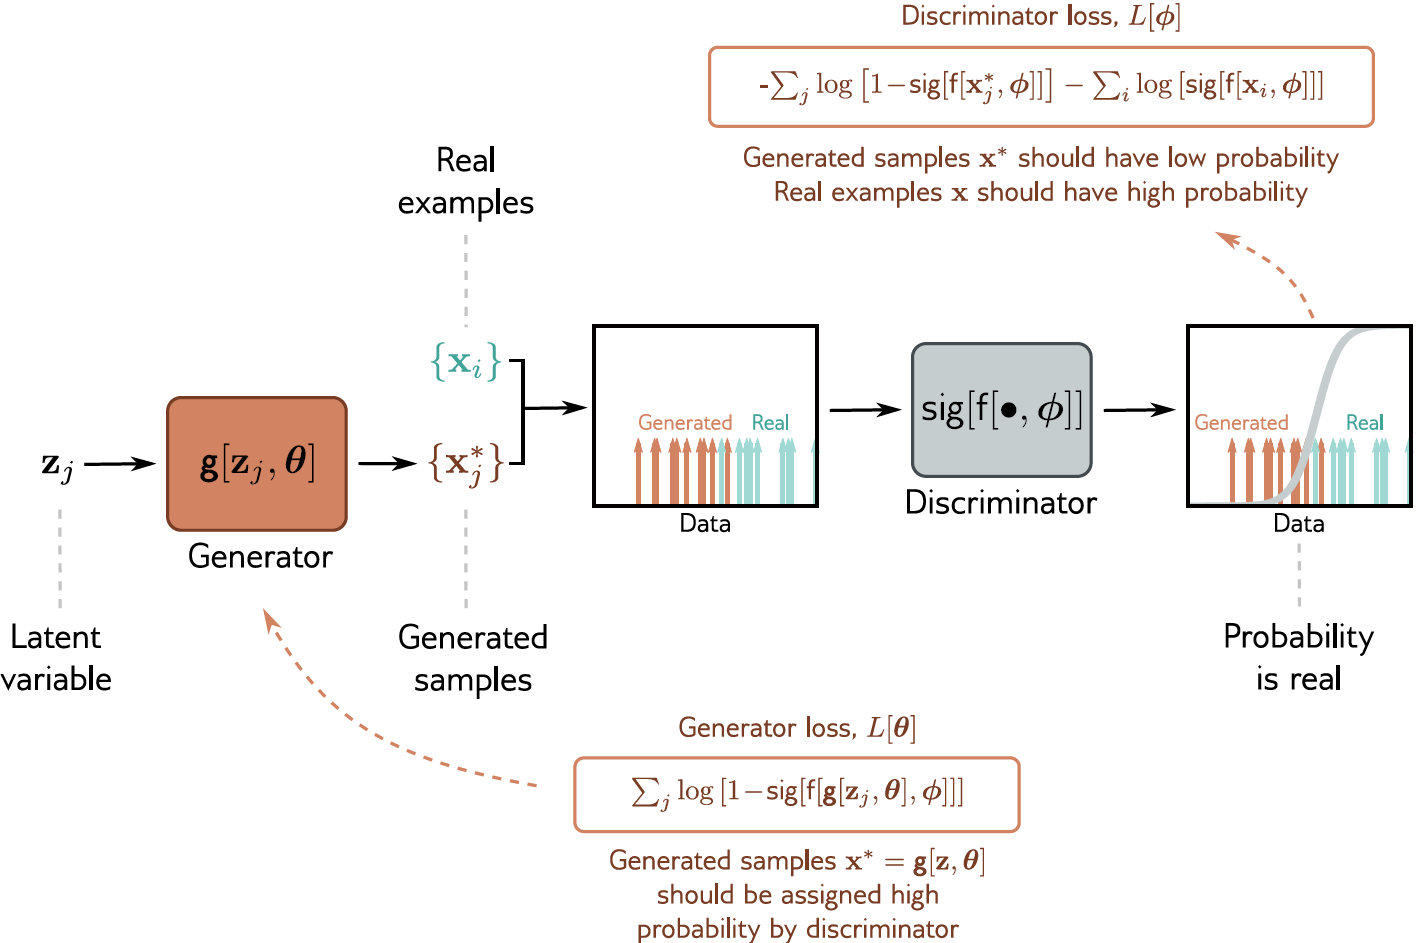
\includegraphics[width=\linewidth]{slides/img/05-geradores/gan-pipeline.png}
      \end{column}
    \end{columns}
  \end{frame}

  %======================================================================
  % SECTION 2: VISÃO GERAL DE NORMALIZING FLOWS
  %======================================================================
  \section{Visão Geral de Normalizing Flows}

  %--- Slide: conceito ---
  \begin{frame}{\textit{Normalizing Flows}\footfullcite{kobyzev2020normalizing}}
    \begin{itemize}
      \item \textit{Normalizing Flows} são modelos geradores
      probabilísticos que permitem \textbf{tanto
      \textcolor{FlowRed}{amostrar} quanto
      \textcolor{FlowRed}{avaliar}} $p_{X}(\mathbf{x})$.
      \item Consistem em \textcolor{AccentBlue}{\textbf{transformar}}
      uma distribuição de base tratável (e.g. $z \sim \mathcal{N}(0,1)$)
      em uma outra distribuição usando \textbf{funções inversíveis}.
    \end{itemize}
    \vspace{0.5em}
    \centering
    \resizebox{0.85\linewidth}{!}{%
      \begin{tikzpicture}[
        box/.style={draw=MediumBlue, fill=PastelGreen, rounded corners=3pt,
                    font=\small, inner sep=10pt, minimum width=1.4cm, align=center},
        ibox/.style={draw=MediumBlue, fill=PastelBlue, rounded corners=3pt,
                     font=\small, inner sep=10pt, minimum width=1.4cm, align=center},
        latent/.style={draw=MediumRed, fill=PastelRed, rounded corners=3pt,
                    font=\small, inner sep=10pt, minimum width=1.0cm},
        arr/.style={->, thick, color=MediumBlue}
      ]
        \node[ibox] (x)  {$\mathbf{x}$};
        \node[box, right=0.9cm of x] (f) {Flow\\$f(\mathbf{x})$};
        \node[latent, right=0.9cm of f] (z) {$\mathbf{z}$};
        \node[ibox, right=0.9cm of z] (fi) {Inverse\\$f^{-1}(\mathbf{z})$};
        \node[ibox, right=0.9cm of fi] (xp) {$\mathbf{x}'$};
        \draw[arr] (x) -- (f);
        \draw[arr] (f) -- (z);
        \draw[arr] (z) -- (fi);
        \draw[arr] (fi) -- (xp);
      \end{tikzpicture}%
    }
    \note{
      A ideia é reaproveitar a simplicidade de uma distribuição base
      (normalmente gaussiana) e deformá-la gradualmente em direção à
      distribuição dos dados, sem perder a capacidade de calcular
      densidades.
    }
  \end{frame}

  %--- Slide: Glow example (marco de 2018) ---
  \begin{frame}{\textit{Normalizing Flows}: o marco de 2018, Glow\footfullcite{kingma2018glow}}
    \centering
    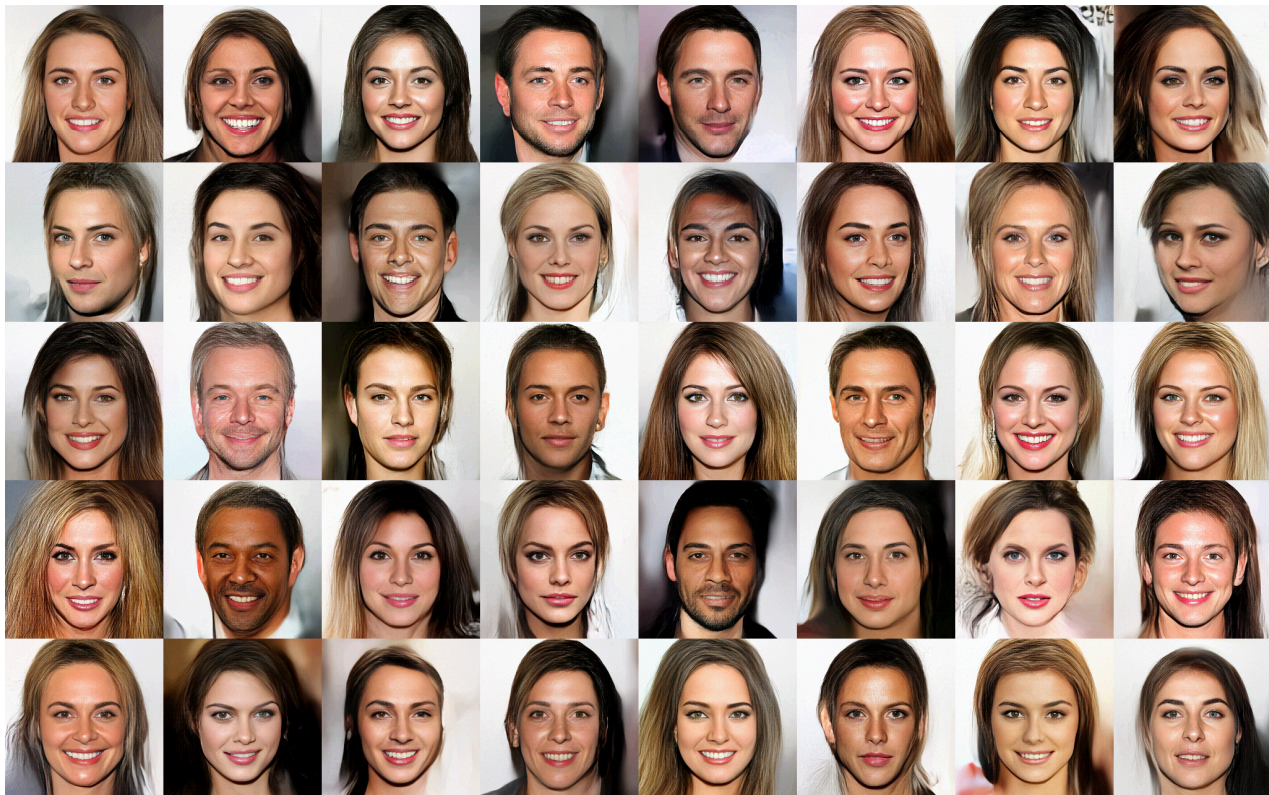
\includegraphics[width=0.46\linewidth]{slides/img/05-geradores/nf-glow-faces.png}\\
    \vspace{0.2em}
    \tiny Faces sintetizadas pelo \textit{Glow} (2018), um \textit{Normalizing
    Flow} com convoluções invertíveis 1{$\times$}1.\par
    \vspace{0.5em}
    \normalsize
    \begin{block}{Durante anos, a referência visual}
      O \textit{Glow} foi durante anos o melhor resultado de imagem de um
      \textit{flow}, firmando a percepção de que NFs ficavam atrás de GANs e
      modelos difusores. Isso mudou a partir de 2024.
    \end{block}
  \end{frame}

  %--- Slide: renascimento dos NFs (2024-2025) ---
  \begin{frame}{O renascimento dos \textit{Normalizing Flows} (2024--2025)}
    Trabalhos recentes mostram NFs  competindo com modelos difusores:
    \vspace{0.4em}
    \centering
    \resizebox{0.96\linewidth}{!}{%
      \begin{tikzpicture}[
        node distance=0.6cm,
        milestone/.style={draw=MediumBlue, fill=PastelBlue, rounded corners=3pt,
                          align=center, font=\small, inner sep=8pt, text width=3.0cm},
        latest/.style={draw=MediumRed, fill=PastelRed, rounded corners=3pt,
                       align=center, font=\small, inner sep=8pt, text width=3.0cm},
        arr/.style={->, thick, color=MediumBlue},
      ]
        \node[milestone] (glow) {\textbf{2018}\\\textit{Glow}\\faces sintéticas};
        \node[milestone, right=of glow] (tar) {\textbf{2024}\\\textit{TarFlow}\\SOTA em \textit{likelihood}};
        \node[latest, right=of tar] (star) {\textbf{2025}\\\textit{STARFlow}\\imagem em alta resolução};
        \node[latest, right=of star] (starv) {\textbf{2025}\\\textit{STARFlow-V}\\geração de vídeo};
        \draw[arr] (glow) -- (tar);
        \draw[arr] (tar) -- (star);
        \draw[arr] (star) -- (starv);
      \end{tikzpicture}%
    }
    \vspace{0.5em}
    \begin{itemize}
      \item \textit{TarFlow}\footfullcite{zhai2025tarflow}: \textit{flow}
      autorregressivo baseado em \textit{Transformer}. Bate o estado da arte
      em verossimilhança de imagens e gera amostras comparáveis às de difusão.
      \item \textit{STARFlow}\footfullcite{gu2025starflow}: escala a ideia
      para síntese em alta resolução no espaço latente.
    \end{itemize}
  \end{frame}

  %--- Slide: 1D transformation ---
  \begin{frame}{\textit{Normalizing Flows}: Transformação 1D}
    Distribuição bimodal dos dados $\leftrightarrow$ gaussiana base via \textit{flow}:
    \vspace{0.3em}
    \centering
    \resizebox{0.92\linewidth}{!}{%
      \begin{tikzpicture}[font=\small]
        % data density (left)
        \begin{axis}[
          name=model,
          width=6cm, height=4cm,
          axis lines=left,
          xmin=-3, xmax=3, ymin=0, ymax=0.8,
          xlabel={$x$}, title={Densidade dos dados $p(x)$},
          xtick=\empty, ytick=\empty,
          clip=false,
        ]
          \addplot[domain=-3:3, samples=120, thick, EncRed, fill=EncRed, fill opacity=0.25]
            {0.55/(sqrt(2*pi)*0.35)*exp(-(x+0.9)^2/(2*0.35^2))
            + 0.45/(sqrt(2*pi)*0.45)*exp(-(x-1.0)^2/(2*0.45^2))} \closedcycle;
        \end{axis}
        % base density (right)
        \begin{axis}[
          at={(model.east)}, xshift=5cm, anchor=west,
          name=base,
          width=6cm, height=4cm,
          axis lines=left,
          xmin=-3, xmax=3, ymin=0, ymax=0.5,
          xlabel={$z$}, title={Densidade base $p(z)$},
          xtick=\empty, ytick=\empty,
          clip=false,
        ]
          \addplot[domain=-3:3, samples=80, thick, DecBlue, fill=DecBlue, fill opacity=0.25]
            {1/(sqrt(2*pi))*exp(-x^2/2)} \closedcycle;
        \end{axis}
        % forward (left -> right) and inverse (right -> left) arrows
        \draw[->, thick, MediumBlue] ($(model.east)+(0.2,0.5)$) -- ($(base.west)+(-0.2,0.5)$)
          node[midway, above, font=\scriptsize] {\textit{Forward} $z = f(x)$};
        \draw[<-, thick, MediumBlue] ($(model.east)+(0.2,-0.2)$) -- ($(base.west)+(-0.2,-0.2)$)
          node[midway, below, font=\scriptsize] {\textit{Inverse} $x = f^{-1}(z)$};
      \end{tikzpicture}%
    }
    \vspace{0.4em}
    \begin{itemize}
      \item \textit{Forward} $f$: leva os dados $p(\mathbf{x})$ para a base $p(\mathbf{z})$
      (avaliação via mudança de variável).
      \item \textit{Inverse} $f^{-1}$: faz o caminho oposto, de $p(\mathbf{z})$ para
      $p(\mathbf{x})$ (amostragem).
    \end{itemize}
    \note{
      A rede aprende os parâmetros de $f$ tais que, quando empurramos
      gaussianas pela rede, saem amostras que se parecem com os dados.
      Como $f$ é inversível, também podemos \emph{perguntar ao modelo}
      qual é a probabilidade de um dado exemplo.
    }
  \end{frame}

  %======================================================================
  % SECTION 3: MUDANÇA DE VARIÁVEL
  %======================================================================
  \section{Mudança de Variável}

  %--- Slide: caso discreto ---
  \begin{frame}{Mudança de Variável: Caso discreto}
    Mudança de variável no caso discreto é \textbf{trivial}. Considere o
    lançamento de um dado:
    \vspace{0.2em}
    \[
      p_{X}(x=1) = \tfrac{1}{6}
    \]
    \vspace{0.2em}
    \begin{itemize}
      \item Aplicando uma função inversível, por exemplo $f(x) = x^{2}$,
      o espaço amostral do experimento muda:
      \[
        \{1, 2, 3, 4, 5, 6\} \;\longrightarrow\; \{1, 4, 9, 16, 25, 36\}
      \]
      \item Para calcularmos $p_{Z}(z = 9)$, basta perceber que
      $z = 9 \equiv x = 3$: \textbf{as probabilidades são iguais}.
    \end{itemize}
    \begin{block}{Caso discreto}
      No discreto, cada evento mantém sua massa de probabilidade: só
      mudam os \emph{rótulos}.
    \end{block}
  \end{frame}

  %--- Slide: caso contínuo - deformação ---
  \begin{frame}{Mudança de Variável: Caso contínuo}
    \begin{columns}[T]
      \begin{column}{0.50\textwidth}
        \begin{itemize}
          \item No contínuo, trabalhamos com
          \textbf{intervalo de probabilidade}, não com evento pontual.
          \item Ao aplicar uma função \textbf{inversível e derivável},
          a densidade sofre uma \textbf{deformação}.
          \item A massa em um volume pode ser \emph{achatada} ou
          \emph{alongada} ao passar pela transformação.
          \item A altura da densidade é \textbf{inversamente
          proporcional} ao alargamento: área total sempre $=1$.
        \end{itemize}
      \end{column}
      \begin{column}{0.46\textwidth}
        \centering
        \resizebox{\linewidth}{!}{%
          \begin{tikzpicture}[font=\small]
            % Eixos x compartilhados: 1 unidade tikz = 1 unidade de dado,
            % origem em tikz x=0 (data 0) nos dois plots.
            % --- Plot de cima: p(z), uniforme em [1,3], altura 0,5 ---
            \draw[->, thick] (0,2.8) -- (4.0,2.8) node[right] {$z$};
            \draw[->, thick] (0,2.8) -- (0,4.3);
            \node[left] at (0,4.2) {$p(z)$};
            \fill[DecBlue, opacity=0.6] (1,2.8) rectangle (3,3.3);
            \node[below, font=\scriptsize] at (1,2.8) {$1$};
            \node[below, font=\scriptsize] at (3,2.8) {$3$};
            \node[left, font=\scriptsize] at (0,3.3) {$.5$};
            % --- Plot de baixo: p(x), uniforme em [0,1], altura 1 ---
            \draw[->, thick] (0,0) -- (4.0,0) node[right] {$x$};
            \draw[->, thick] (0,0) -- (0,1.5);
            \node[left] at (0,1.4) {$p(x)$};
            \fill[ReconGreen, opacity=0.6] (0,0) rectangle (1,1);
            \node[below, font=\scriptsize] at (0,0) {$0$};
            \node[below, font=\scriptsize] at (1,0) {$1$};
            \node[left, font=\scriptsize] at (0,1) {$1$};
            % --- Setas mostrando o alongamento via f(x)=2x+1 ---
            \foreach \xs/\xt in {0/1, 0.25/1.5, 0.5/2, 0.75/2.5, 1/3}{
              \draw[->, EncRed, thick] (\xs,1.05) -- (\xt,2.75);
            }
            \node[EncRed, font=\scriptsize, anchor=west] at (3.2,2.05) {$f(x) = 2x+1$};
            \node[EncRed, font=\scriptsize, anchor=west] at (3.2,1.55) {$f^{-1}(z) = \tfrac{z-1}{2}$};
          \end{tikzpicture}%
        }\\
        \tiny Uniforme $p(x)$ transformada em $p(z)$ mais larga e menos
        alta por $z = 2x+1$.
      \end{column}
    \end{columns}
    \note{
      Observação didática: se o intervalo duplica de largura, a altura
      tem que ser cortada pela metade para preservar a área. É
      exatamente esse fator de escala (o módulo do Jacobiano) que
      aparece na fórmula de mudança de variável.
    }
  \end{frame}

  %--- Slide: equação base ---
  \begin{frame}{Mudança de Variável: Equação base}
    A conservação de probabilidade exige que infinitesimais de
    probabilidade se preservem:
    \vspace{0.6em}
    \[
      p(x)\, dx = p(z)\, dz
    \]
    \vspace{0.2em}
    \begin{itemize}
      \item Isso é a regra da mudança de variável em
      densidades.
      \item Intuitivamente: a \emph{área sob a curva} em um intervalo
      transformado deve ser igual à área no intervalo original.
    \end{itemize}
  \end{frame}

  %--- Slide: equação com módulo ---
  \begin{frame}{Mudança de Variável: Fórmula explícita}
    Reorganizando, expressamos $p(x)$ em função de $p(z)$:
    \vspace{0.3em}
    \[
      p(x)\, dx = p(z)\, dz
      \quad\Longrightarrow\quad
      p(x) = p(z) \left|\dfrac{dz}{dx}\right|
    \]
    \vspace{0.3em}
    \begin{block}{Por que o módulo?}
      Se $f$ é decrescente, $dz/dx < 0$ e o intervalo $[x, x+dx]$ é levado
      a $[z+dz, z]$, com a orientação invertida. O módulo absorve esse
      sinal: a massa no intervalo é a mesma e a densidade resultante fica
      não negativa.
    \end{block}
  \end{frame}

  %--- Slide: exemplo explícito (enunciado + figura) ---
  \begin{frame}{Mudança de Variável: exemplo log-normal}
    \textbf{Setup:} base $Z \sim \mathcal{N}(0,1)$ e dados $X = \exp(Z)$.
    Qual é a densidade $p_{X}(x)$?
    \vspace{0.2em}
    \begin{center}
      \resizebox{!}{0.72\textheight}{%
      \begin{tikzpicture}[font=\small]
        % --- Centro (canto inferior direito): função z = exp(x), x vertical, z horizontal ---
        \begin{axis}[
          name=expfn,
          width=6.2cm, height=4.4cm,
          axis lines=left,
          xmin=0, xmax=12, ymin=-2.5, ymax=2.5,
          xlabel={$x$},
          xlabel style={font=\scriptsize},
          xtick={2,4,6,8,10,12}, ytick={-2,-1,0,1,2},
          tick label style={font=\scriptsize},
          clip=false,
        ]
          % Curva paramétrica: (z = exp(x), x) com x na vertical
          \addplot[domain=-2.5:2.5, samples=120, thick, EncRed]
            ({exp(x)}, x);
          \node[EncRed, font=\scriptsize, anchor=south east] at (axis cs:11.5,-2.2) {$x = \exp(z)$};
          % Linha de tracejado: x = 0 -> z = 1
          \draw[dashed, FlowGreen, thick] (axis cs:0,0) -- (axis cs:1,0);
          \draw[dashed, FlowGreen, thick] (axis cs:1,0) -- (axis cs:1,2.5);
        \end{axis}
        % --- Esquerda (canto inferior esquerdo): Normal(0,1) rotacionada, x vertical, densidade horizontal ---
        \begin{axis}[
          at={(expfn.south west)}, anchor=south east, xshift=-0.4cm,
          name=normal,
          width=4.2cm, height=4.4cm,
          axis lines=left,
          xmin=0, xmax=0.5, ymin=-2.5, ymax=2.5,
          xlabel={$p_Z(z)$}, ylabel={$z$},
          xlabel style={font=\scriptsize}, ylabel style={font=\scriptsize},
          xtick={0.1,0.3,0.5}, ytick={-2,-1,0,1,2},
          tick label style={font=\scriptsize},
          clip=false,
        ]
          \addplot[domain=-2.5:2.5, samples=100, thick, DecBlue, fill=DecBlue, fill opacity=0.25]
            ({1/sqrt(2*pi)*exp(-x^2/2)}, x) \closedcycle;
          \node[DecBlue, font=\scriptsize, anchor=south east] at (axis cs:0.48,1.5) {$\mathcal{N}(0,1)$};
          % Linha de tracejado: indica x = 0 (modo)
          \draw[dashed, FlowGreen, thick] (axis cs:0,0) -- (axis cs:0.4,0);
        \end{axis}
        % --- Cima (canto superior direito): log-normal, z horizontal, densidade vertical ---
        \begin{axis}[
          at={(expfn.north west)}, anchor=south west, yshift=0.4cm,
          name=lognorm,
          width=6.2cm, height=3.6cm,
          axis lines=left,
          xmin=0, xmax=12, ymin=0, ymax=0.7,
          xlabel={$x$},
          xlabel style={font=\scriptsize},
          xtick={2,4,6,8,10,12}, ytick={0.2,0.4,0.6},
          tick label style={font=\scriptsize},
          clip=false,
        ]
          \addplot[domain=0.05:12, samples=240, thick, ReconGreen, fill=ReconGreen, fill opacity=0.25]
            {1/(x*sqrt(2*pi))*exp(-(ln(x))^2/2)} \closedcycle;
          \node[ReconGreen, font=\scriptsize, anchor=north east] at (axis cs:11.5,0.65) {$p_X(x)$: log-normal};
          % Linha de tracejado: z = 1
          \draw[dashed, FlowGreen, thick] (axis cs:1,0) -- (axis cs:1,0.4);
        \end{axis}
      \end{tikzpicture}}
    \end{center}
  \end{frame}

  %--- Slide: exemplo explícito (solução) ---
  \begin{frame}{Mudança de Variável: Solução log-normal}
    \begin{block}{Passos}
      \begin{enumerate}
        \item Densidade da base:
        $p_{Z}(z) = \tfrac{1}{\sqrt{2\pi}}\exp\!\left(-\tfrac{z^{2}}{2}\right)$.
        \item Como $x = \exp(z)$, o \textit{flow} que leva dados à base é
        $z = f(x) = \ln x$.
        \item $P(X \leq x) = P(Z \leq \ln x)$, logo
        $\mathrm{CDF}_X(x) = \mathrm{CDF}_Z(\ln x)$; derivando,
        $p_{X}(x) = p_{Z}(\ln x)\,\tfrac{\partial (\ln x)}{\partial x}$.
        \item Substituindo $p_{Z}(\ln x)$ e $\tfrac{\partial (\ln x)}{\partial x} = \tfrac{1}{x}$:
        \vspace{-0.6em}
        {\small
        \begin{align*}
          p_{X}(x)
            &= \underbrace{\tfrac{1}{\sqrt{2\pi}}\exp\!\left(-\tfrac{(\ln x)^{2}}{2}\right)}_{p_{Z}(\ln x)}
               \cdot
               \underbrace{\tfrac{1}{x}}_{\partial (\ln x)/\partial x}
             = \tfrac{1}{x\sqrt{2\pi}}\exp\!\left(-\tfrac{(\ln x)^{2}}{2}\right).
        \end{align*}}%
        \vspace{-0.8em}
        \item Essa é a densidade \textbf{log-normal}, obtida pela fórmula
        $p_X(x) = p_Z(f(x))\,|f'(x)|$ com $f = \ln$ e $|f'(x)| = 1/x$.
      \end{enumerate}
    \end{block}
  \end{frame}

  %--- Slide: caso multidimensional ---
  \begin{frame}{Mudança de Variável: Caso multidimensional}
    Em mais de uma dimensão, a derivada $\left|\tfrac{dz}{dx}\right|$ vira o
    \textbf{módulo do determinante da matriz Jacobiana}:
    \vspace{0.3em}
    \[
      p_X(\mathbf{x}) = p_Z(\mathbf{z})\left|\det \tfrac{\partial \mathbf{z}}{\partial \mathbf{x}}\right|
      = p_Z(\mathbf{z})\left|\det \tfrac{\partial f(\mathbf{x})}{\partial \mathbf{x}}\right|,
      \qquad \mathbf{z} = f(\mathbf{x}).
    \]
    \vspace{0.2em}
    \begin{itemize}
      \item O caso 1D já visto é um caso particular (determinante de uma
      matriz $1{\times}1$).
      \item Em logaritmo (forma que aparece na \emph{loss} a seguir):
      \[
        \log p_X(\mathbf{x}) = \log p_Z(f(\mathbf{x}))
        + \log\left|\det \tfrac{\partial f(\mathbf{x},\thetav)}{\partial \mathbf{x}}\right|.
      \]
      \item Treinar $=$ empurrar os dados por $f$ até $\mathbf{z}$ e
      acumular o \textbf{log-determinante}.
    \end{itemize}
  \end{frame}

  %======================================================================
  % SECTION 4: LOSS
  %======================================================================
  \section{Loss}

  %--- Slide: verossimilhança ---
  \begin{frame}{Loss: \textit{Maximum Likelihood}}
    Para treinar, seguimos o \textit{framework} de maximizar a
    \textbf{verossimilhança} dos dados:
    \vspace{0.3em}
    \[
      \hat{\thetav} = \argmax_{\thetav}
      \left[\prod_{i=1}^{N} p_X\!\left(\mathbf{x}^{(i)} \mid \thetav\right)\right]
    \]
    \vspace{0.2em}
    \begin{itemize}
      \item O produto vem da suposição de independência das amostras.
      \item Usualmente trabalhamos com a log-verossimilhança (soma, não
      produto) e a minimizamos com sinal trocado.
    \end{itemize}
  \end{frame}

  %--- Slide: derivação NLL - passo 1 ---
  \begin{frame}{Loss: NLL passo a passo (1/2)}
    \textbf{Passo 1}: trocamos produto por soma negativa (NLL):
    \vspace{0.3em}
    \begin{align*}
      \hat{\thetav}
      &= \argmax_{\thetav}\left[\prod_{i} p_X(\mathbf{x}^{(i)}\mid\thetav)\right]
      \\[0.2em]
      &\visible<2->{= \argmin_{\thetav}
        \left[\sum_{i=1}^{N} -\log p_X\!\left(\mathbf{x}^{(i)} \mid \thetav\right)\right]}
    \end{align*}
    \vspace{0.3em}
    \only<1>{\emph{Produtos de muitas probabilidades pequenas sofrem
    \textit{underflow} numérico. Aplicando o logaritmo, o produto vira
    soma e a otimização fica estável.}}
    \only<2->{
      \begin{block}{Mudança de variável do \textit{flow}}
      \vspace{-0.5em}
        \[
          p_X(\mathbf{x}) = p_Z(\mathbf{z})\left|\det \tfrac{\partial f(\mathbf{x},\thetav)}{\partial \mathbf{x}}\right|,
          \quad \mathbf{z} = f(\mathbf{x},\thetav)
        \]
      \end{block}
      \emph{Vamos substituir $p_X(\mathbf{x}^{(i)}\mid \thetav)$ na expressão
      acima.}
    }
    \note{
      Observação: NLL = sempre mínimo, sempre bem-definido
      numericamente. Log vira nossos produtos em somas e nossas
      divisões em subtrações.
    }
  \end{frame}

  %--- Slide: derivação NLL - passo 2 ---
  \begin{frame}{Loss: NLL passo a passo (2/2)}
    \textbf{Passo 2}: substituir $p_X$ pela mudança de variável, com
    $\mathbf{z}^{(i)} = f(\mathbf{x}^{(i)},\thetav)$:
    \vspace{0.3em}
    \begin{align*}
      \hat{\thetav}
      &\visible<1->{= \argmin_{\thetav}
        \left[\sum_{i=1}^{N} -\log\!\left(p_Z(\mathbf{z}^{(i)})\left|\det \tfrac{\partial f(\mathbf{x}^{(i)},\thetav)}{\partial \mathbf{x}^{(i)}}\right|\right)\right]} \\[0.2em]
      &\visible<2->{= \argmin_{\thetav}
        \left[\sum_{i=1}^{N}\!\left[-\log\!\left|\det \tfrac{\partial f(\mathbf{x}^{(i)},\thetav)}{\partial \mathbf{x}^{(i)}}\right| - \log p_Z(\mathbf{z}^{(i)})\right]\right]}
    \end{align*}
    \vspace{0.3em}
    \visible<2->{
      \begin{alertblock}{Dois termos, dois papéis}
        \begin{itemize}
          \item \textcolor{EncRed}{$-\log\left|\det \tfrac{\partial f}{\partial \mathbf{x}}\right|$}: depende de
          $\thetav$ via a rede. Mede a deformação local de volume
          induzida pelo \textit{flow}.
          \item \textcolor{DecBlue}{$-\log p_Z(\mathbf{z})$}: a distribuição base é
          fixa (gaussiana), com densidade em forma fechada. $\thetav$
          entra apenas através de $\mathbf{z} = f(\mathbf{x},\thetav)$.
        \end{itemize}
      \end{alertblock}
    }
    \note{
      O aluno deve sair com a intuição: \emph{o log-determinante da
      Jacobiana é o ``preço'' pago em termos de compressão de volume,
      e aparece naturalmente na NLL.}
    }
  \end{frame}

  %======================================================================
  % SECTION 5: O QUE SÃO FLOWS
  %======================================================================
  \section{O que são Flows}

  %--- Slide: definição ---
  \begin{frame}{\textit{Flows}}
    Um \textit{flow} é uma função $f(\mathbf{x})$ com quatro
    propriedades:
    \vspace{0.4em}
    \begin{itemize}
      \item \textbf{Paramétrica}: queremos definir parâmetros
      aprendíveis.
      \item \textcolor{FlowGreen}{\textbf{Inversível}}: queremos
      calcular o \textit{flow} nos dois sentidos (amostragem e
      avaliação).
      \item \textbf{Diferenciável}: queremos otimizar via
      \textit{backprop}.
      \item \textbf{Jacobiana tratável}: conseguimos computar a
      inversa e o determinante da Jacobiana de \textbf{maneira
      eficiente}.
    \end{itemize}
    \begin{alertblock}{Desafio de engenharia}
      Satisfazer os quatro requisitos simultaneamente é o que define
      um \textit{flow}.
    \end{alertblock}
  \end{frame}

  %--- Slide: composição ---
  \begin{frame}{\textit{Flows}: Composição}
    A classe de funções diferenciáveis e inversíveis é \textbf{fechada
    em composição}:
    \vspace{0.3em}
    \[
      f = f_{k} \circ f_{k-1} \circ \cdots \circ f_{2} \circ f_{1}
    \]
    \vspace{0.3em}
    \begin{itemize}
      \item Isso nos possibilita \textbf{projetar camadas} que computam
      um \textit{flow} e empilhá-las em redes profundas.
      \item A expressividade vem da composição: cada camada pode ser
      simples desde que a composição seja rica.
    \end{itemize}
  \end{frame}

  %--- Slide: diagrama composição ---
  \begin{frame}{\textit{Flows}: Normalização e geração}
    \centering
    \resizebox{0.95\linewidth}{!}{%
      \begin{tikzpicture}[
          fwd/.style={->, thick, FlowGreen},
          inv/.style={->, thick, black!55},
        ]
        % --- cinco densidades: dados (esq.) -> base (dir.) ---
        \draw[domain=-1.3:1.3, samples=80, DecBlue, thick]
          plot ({\x+0},{0.8*exp(-(\x+0.8)^2/0.12)+0.8*exp(-(\x)^2/0.12)+0.8*exp(-(\x-0.8)^2/0.12)});
        \draw[domain=-1.3:1.3, samples=60, DecBlue, thick]
          plot ({\x+3},{0.85*exp(-(\x+0.5)^2/0.18)+0.85*exp(-(\x-0.5)^2/0.18)});
        \draw[domain=-1.3:1.3, samples=60, DecBlue, thick]
          plot ({\x+6},{0.8*exp(-(\x+0.3)^2/0.3)+0.5*exp(-(\x-0.7)^2/0.18)});
        \draw[domain=-1.3:1.3, samples=60, DecBlue, thick]
          plot ({\x+9},{0.9*exp(-(\x-0.1)^2/0.5)+0.18*exp(-(\x-0.7)^2/0.15)});
        \draw[domain=-1.3:1.3, samples=60, DecBlue, thick]
          plot ({\x+12},{exp(-(\x)^2/0.5)});
        \node[font=\scriptsize] at (0,1.35)  {dados $p(\mathbf{x})$};
        \node[font=\scriptsize] at (12,1.35) {base $p(\mathbf{z})$};
        % --- normalização (verde, esq. -> dir.) e geração (cinza, dir. -> esq.) ---
        \draw[fwd] (-1.0,2.6) -- (13.0,2.6)
          node[midway, above, font=\small, FlowGreen] {$f = f_{4}\circ f_{3}\circ f_{2}\circ f_{1}$};
        \draw[inv] (13.0,-1.4) -- (-1.0,-1.4)
          node[midway, below, font=\small]
          {$f^{-1} = f_{1}^{-1}\circ f_{2}^{-1}\circ f_{3}^{-1}\circ f_{4}^{-1}$};
        \foreach \gx/\lab in {1.5/1, 4.5/2, 7.5/3, 10.5/4}{
          \draw[fwd] (\gx-0.8,1.75) -- (\gx+0.8,1.75)
            node[midway, above, font=\scriptsize, FlowGreen] {$f_{\lab}$};
          \draw[inv] (\gx+0.8,-0.4) -- (\gx-0.8,-0.4)
            node[midway, below, font=\scriptsize, black!55] {$f_{\lab}^{-1}$};
        }
      \end{tikzpicture}%
    }\\
    \vspace{0.3em}
    \begin{itemize}
      \item Normalização ($f = f_{4} \circ f_{3} \circ f_{2} \circ f_{1}$):
      leva os dados $p(\mathbf{x})$ à base $p(\mathbf{z})$ (verde).
      \item Geração ($f^{-1} = f_{1}^{-1} \circ f_{2}^{-1} \circ f_{3}^{-1} \circ f_{4}^{-1}$):
      o caminho inverso, da base $p(\mathbf{z})$ aos dados $p(\mathbf{x})$ (cinza).
    \end{itemize}
  \end{frame}

  %--- Slide: Jacobian da composição ---
  \begin{frame}{\textit{Flows}: Jacobiana da composição}
    Pela regra da cadeia, o determinante da Jacobiana de uma composição
    é o \textbf{produto dos determinantes}:
    \vspace{0.3em}
    \[
      \left|\frac{\partial f[\mathbf{x},\thetav]}{\partial \mathbf{x}}\right|
      = \left|\frac{\partial f_{k}[f_{k-1},\thetav_k]}{\partial f_{k-1}}\right|
      \cdot
      \left|\frac{\partial f_{k-1}[f_{k-2},\thetav_{k-1}]}{\partial f_{k-2}}\right|
      \cdots
      \left|\frac{\partial f_{1}[\mathbf{x},\thetav_1]}{\partial \mathbf{x}}\right|
    \]
    \vspace{0.3em}
    \begin{itemize}
      \item Por isso, basta que cada camada tenha Jacobiana \emph{fácil
      de calcular} para que a rede inteira também tenha.
      \item Esse é o princípio que guia o design de arquiteturas de
      \textit{flows}.
    \end{itemize}
  \end{frame}

  %--- Slide: linear flow ---
  \begin{frame}{\textit{Linear Flow}}
    Uma transformação \textbf{linear} pode ser um \textit{Linear Flow}
    se a matriz admitir inversa:
    \vspace{0.3em}
    \[
      f(\mathbf{x}) = \mathbf{x}\,\mathbf{\Theta}^{\top} + \mathbf{b}
      \qquad
      f^{-1}(\mathbf{z}) = (\mathbf{z} - \mathbf{b})\,(\mathbf{\Theta}^{\top})^{-1}
    \]
    \vspace{0.3em}
    \begin{alertblock}{Problemas}
      \begin{itemize}
        \item \textbf{Pouco expressiva}: uma transformação linear de uma
        gaussiana continua gaussiana, então o modelo nunca sai da família
        da base (e compor lineares continua linear).
        \item Determinante e inversa de matriz densa: custo
        $\mathcal{O}(d^{3})$.
      \end{itemize}
    \end{alertblock}
  \end{frame}

  %--- Slide: linear flow table ---
  \begin{frame}{\textit{Linear Flow}: Custo por estrutura}
    Impondo estrutura na matriz $\mathbf{\Theta}$, reduzimos drasticamente o custo
    de inverter e de calcular o determinante. \emph{Diagonal} é barata mas muito
    restritiva; \textcolor{EncRed}{\emph{LU factorized}} e
    \textcolor{EncRed}{\emph{$1{\times}1$ convolution}} são os \textit{linear
    flows} usados no Glow, alternados com \textit{coupling layers}.
    \vspace{0.4em}
    \begin{center}
      \footnotesize
      \renewcommand{\arraystretch}{1.25}
      \begin{tabular}{lcc}
        \toprule
        \textbf{Estrutura} & \textbf{Inversa} & \textbf{Determinante} \\
        \midrule
        Full           & $\mathcal{O}(d^{3})$   & $\mathcal{O}(d^{3})$   \\
        Diagonal       & $\mathcal{O}(d)$       & $\mathcal{O}(d)$       \\
        Triangular     & $\mathcal{O}(d^{2})$   & $\mathcal{O}(d)$       \\
        Block Diagonal & $\mathcal{O}(c^{3} d)$ & $\mathcal{O}(c^{3} d)$ \\
        \textcolor{EncRed}{LU Factorized}
                       & \textcolor{EncRed}{$\mathcal{O}(d^{2})$}
                       & \textcolor{EncRed}{$\mathcal{O}(d)$}           \\
        Spatial Convolution & $\mathcal{O}(d \log d)$ & $\mathcal{O}(d)$ \\
        \textcolor{EncRed}{$1{\times}1$ Convolution}
                       & \textcolor{EncRed}{$\mathcal{O}(c^{3} + c^{2} d)$}
                       & \textcolor{EncRed}{$\mathcal{O}(c^{3})$}       \\
        \bottomrule
      \end{tabular}
    \end{center}
    \vspace{0.1em}
    \tiny LU \textit{factorized} e \textit{spatial}/$1{\times}1$ convolution:
    Kingma \& Dhariwal (2018); Hoogeboom et al.\ (2019). $d$: dimensão;
    $c$: canais.\par
  \end{frame}

  %======================================================================
  % SECTION 6: COUPLING FLOWS
  %======================================================================
  \section{Coupling Flows}

  %--- Slide: coupling forward ---
  \begin{frame}{\textit{Coupling Flows}\footfullcite{dinh2017realnvp}}
    \small
    Dividir a entrada em duas metades e transformar apenas uma delas,
    \emph{condicionando na outra}:
    \vspace{0.2em}
    \[
      \mathbf{z} = f(\mathbf{x}) = \begin{bmatrix}
        \mathbf{x}^{A} \\
        \hat{f}\!\left(\mathbf{x}^{B} \mid \thetav(\mathbf{x}^{A})\right)
      \end{bmatrix}
    \]
    \vspace{0.2em}
    \centering
    \resizebox{0.78\linewidth}{!}{%
      \begin{tikzpicture}[
          font=\small,
          cell/.style={draw=MediumBlue, thick, minimum width=0.7cm, minimum height=0.55cm, inner sep=1pt},
          acell/.style={cell, fill=PastelBlue},
          bcell/.style={cell, fill=PastelGreen},
          rcell/.style={cell, fill=PastelRed},
          box/.style={draw=MediumBlack, thick, rounded corners=2pt, fill=white,
                      align=center, font=\scriptsize, inner sep=4pt},
          fwd/.style={->, thick, MediumBlue},
          cpy/.style={->, thick, black!50},
        ]
        % entrada x
        \node[acell] (x1) at (0,2.70) {}; \node[acell] (x2) at (0,2.10) {};
        \node[bcell] (x3) at (0,1.50) {}; \node[bcell] (x4) at (0,0.90) {};
        \node at (0,3.30) {$\mathbf{x}$};
        % split
        \node[acell] (a1) at (3,3.00) {}; \node[acell] (a2) at (3,2.40) {};
        \node[bcell] (b1) at (3,1.20) {}; \node[bcell] (b2) at (3,0.60) {};
        \node[font=\scriptsize] at (3,3.55) {$\mathbf{x}^{A}$};
        \node[font=\scriptsize] at (3,0.05) {$\mathbf{x}^{B}$};
        % caixas
        \node[box] (cn) at (6,2.05) {Coupling\\Network $\thetav(\mathbf{x}^{A})$};
        \node[box] (ct) at (6,0.50) {Coupling\\Transform};
        % saida
        \node[acell] (f1) at (9.6,2.70) {}; \node[acell] (f2) at (9.6,2.10) {};
        \node[rcell] (f3) at (9.6,1.50) {}; \node[rcell] (f4) at (9.6,0.90) {};
        \node at (9.6,3.30) {$\mathbf{z} = f(\mathbf{x})$};
        % legenda de cores
        \node[acell, minimum width=0.45cm, minimum height=0.32cm] (l1) at (0.3,-0.65) {};
        \node[right=2pt of l1, font=\scriptsize] {$\mathbf{x}^{A}$, copiado};
        \node[bcell, minimum width=0.45cm, minimum height=0.32cm] (l2) at (3.6,-0.65) {};
        \node[right=2pt of l2, font=\scriptsize] {$\mathbf{x}^{B}$, entrada da \textit{transform}};
        \node[rcell, minimum width=0.45cm, minimum height=0.32cm] (l3) at (7.6,-0.65) {};
        \node[right=2pt of l3, font=\scriptsize] {$\mathbf{z}^{B}$, transformado};
        % split arrows
        \draw[cpy] (x1.east) -- (a1.west); \draw[cpy] (x2.east) -- (a2.west);
        \draw[cpy] (x3.east) -- (b1.west); \draw[cpy] (x4.east) -- (b2.west);
        \node[font=\scriptsize, black!60] at (1.5,3.20) {Split};
        % A -> network
        \draw[fwd] (3.5,2.20) -- (cn.west);
        % A copiado (arco)
        \draw[cpy] (a1.east) .. controls (6,3.55) .. (f1.west);
        \node[font=\scriptsize, black!60] at (6,3.62) {cópia $\mathbf{x}^{A}$};
        \draw[cpy] (a2.east) .. controls (6,3.10) .. (f2.west);
        % B -> transform
        \draw[fwd] (b1.east) -- (ct.west); \draw[fwd] (b2.east) -- (ct.west);
        % network -> transform
        \draw[fwd] (cn.south) -- (ct.north) node[midway, right, font=\scriptsize] {$\thetav(\mathbf{x}^{A})$};
        % transform -> saida
        \draw[fwd] (ct.east) -- (f3.west); \draw[fwd] (ct.east) -- (f4.west);
        \node[font=\scriptsize, black!60] at (8.0,1.95) {Concat.};
      \end{tikzpicture}%
    }
  \end{frame}

  %--- Slide: coupling inverse ---
  \begin{frame}{\textit{Coupling Flows}: Inversa}
    Como $\mathbf{x}^{A}$ é copiado direto, temos
    $\mathbf{z}^{A} = \mathbf{x}^{A}$. Para inverter basta aplicar
    $\hat{f}^{-1}$ em $\mathbf{z}^{B}$ usando a mesma \textit{coupling
    network} que produziu os parâmetros:
    \vspace{0.3em}
    \[
      f^{-1}(\mathbf{z}) = \begin{bmatrix}
        \mathbf{z}^{A} \\
        \hat{f}^{-1}\!\left(\mathbf{z}^{B} \mid \thetav(\mathbf{z}^{A})\right)
      \end{bmatrix}
    \]
    \vspace{0.2em}
    \centering
    \resizebox{0.84\linewidth}{!}{%
      \begin{tikzpicture}[
          font=\small,
          cell/.style={draw=MediumBlue, thick, minimum width=0.7cm, minimum height=0.55cm, inner sep=1pt},
          acell/.style={cell, fill=PastelBlue},
          bcell/.style={cell, fill=PastelGreen},
          rcell/.style={cell, fill=PastelRed},
          box/.style={draw=MediumBlack, thick, rounded corners=2pt, fill=white,
                      align=center, font=\scriptsize, inner sep=4pt},
          inv/.style={->, thick, MediumGreen},
          cpy/.style={->, thick, black!50},
        ]
        % entrada z (direita)
        \node[acell] (z1) at (9.6,2.70) {}; \node[acell] (z2) at (9.6,2.10) {};
        \node[rcell] (z3) at (9.6,1.50) {}; \node[rcell] (z4) at (9.6,0.90) {};
        \node at (9.6,3.30) {$\mathbf{z}$};
        % split
        \node[acell] (a1) at (6.6,3.00) {}; \node[acell] (a2) at (6.6,2.40) {};
        \node[rcell] (b1) at (6.6,1.20) {}; \node[rcell] (b2) at (6.6,0.60) {};
        \node[font=\scriptsize] at (6.6,3.55) {$\mathbf{z}^{A}$};
        \node[font=\scriptsize] at (6.6,0.05) {$\mathbf{z}^{B}$};
        % caixas
        \node[box] (cn) at (3.6,2.05) {Coupling\\Network $\thetav(\mathbf{z}^{A})$};
        \node[box] (ct) at (3.6,0.50) {Inverse\\Transform};
        % saida (esquerda)
        \node[acell] (f1) at (0,2.70) {}; \node[acell] (f2) at (0,2.10) {};
        \node[bcell] (f3) at (0,1.50) {}; \node[bcell] (f4) at (0,0.90) {};
        \node at (0,3.30) {$f^{-1}(\mathbf{z})$};
        % split arrows (direita -> esquerda)
        \draw[cpy] (z1.west) -- (a1.east); \draw[cpy] (z2.west) -- (a2.east);
        \draw[cpy] (z3.west) -- (b1.east); \draw[cpy] (z4.west) -- (b2.east);
        \node[font=\scriptsize, black!60] at (8.1,3.20) {Split};
        % A reavalia a network
        \draw[inv] (6.1,2.20) -- (cn.east);
        % A copiado (arco)
        \draw[cpy] (a1.west) .. controls (3.6,3.55) .. (f1.east);
        \node[font=\scriptsize, black!60] at (3.6,3.62) {cópia $\mathbf{z}^{A}$};
        \draw[cpy] (a2.west) .. controls (3.6,3.10) .. (f2.east);
        % B -> inverse transform
        \draw[inv] (b1.west) -- (ct.east); \draw[inv] (b2.west) -- (ct.east);
        % network -> transform
        \draw[inv] (cn.south) -- (ct.north) node[midway, right, font=\scriptsize] {$\thetav(\mathbf{z}^{A})$};
        % transform -> saida
        \draw[inv] (ct.west) -- (f3.east); \draw[inv] (ct.west) -- (f4.east);
        \node[font=\scriptsize, black!60] at (1.6,1.95) {Concat.};
      \end{tikzpicture}%
    }
  \end{frame}

  %--- Slide: coupling with permutation ---
  \begin{frame}{\textit{Coupling Flows}: Combinando com permutações}
    Um único \textit{coupling layer} só transforma metade das dimensões.
    \textbf{Alternando permutações} (ou \textit{linear flows}) entre as
    camadas, todas as dimensões são afetadas:
    \vspace{0.2em}
    \centering
    \resizebox{0.70\linewidth}{!}{%
      \begin{tikzpicture}[
          font=\small,
          cell/.style={draw=MediumBlue, thick, minimum width=0.62cm, minimum height=0.5cm, inner sep=1pt},
          box/.style={draw=MediumBlack, thick, rounded corners=2pt, fill=white,
                      align=center, font=\scriptsize, inner sep=4pt},
          fwd/.style={->, thick, MediumBlue},
          cpy/.style={->, thick, black!50},
        ]
        % entrada x (4 dimensões coloridas)
        \node[cell, fill=orange!35]   (x1) at (0,2.55) {};
        \node[cell, fill=PastelGreen] (x2) at (0,2.00) {};
        \node[cell, fill=PastelBlue]  (x3) at (0,1.45) {};
        \node[cell, fill=violet!30]   (x4) at (0,0.90) {};
        \node at (0,3.15) {$\mathbf{x}$};
        % permutação
        \node[box, minimum height=2.1cm, text width=1.3cm] (perm) at (2.2,1.72)
          {Permu-\\tation /\\Linear};
        % permutado e dividido
        \node[cell, fill=PastelBlue]  (p1) at (4.4,2.85) {};
        \node[cell, fill=violet!30]   (p2) at (4.4,2.30) {};
        \node[cell, fill=orange!35]   (p3) at (4.4,1.15) {};
        \node[cell, fill=PastelGreen] (p4) at (4.4,0.60) {};
        \node[font=\scriptsize] at (4.4,3.35) {$\mathbf{x}^{A}$};
        \node[font=\scriptsize] at (4.4,0.10) {$\mathbf{x}^{B}$};
        \node[font=\scriptsize, black!60] at (3.55,3.05) {Split};
        % caixas
        \node[box] (cn) at (6.9,2.05) {Coupling\\Network};
        \node[box] (ct) at (6.9,0.55) {Coupling\\Transform};
        % saida
        \node[cell, fill=PastelBlue] (f1) at (9.6,2.55) {};
        \node[cell, fill=violet!30]  (f2) at (9.6,2.00) {};
        \node[cell, fill=PastelRed]  (f3) at (9.6,1.45) {};
        \node[cell, fill=PastelRed]  (f4) at (9.6,0.90) {};
        \node at (9.6,3.15) {$\mathbf{z}$};
        \node[font=\scriptsize, black!60] at (8.5,2.95) {Concat.};
        % fluxos
        \draw[fwd] (0.4,1.72) -- (perm.west);
        \draw[fwd] (perm.east) -- (3.9,1.72);
        \draw[fwd] (4.9,2.55) -- (cn.west);
        \draw[cpy] (p1.east) .. controls (6.9,3.45) .. (f1.west);
        \draw[cpy] (p2.east) .. controls (6.9,3.00) .. (f2.west);
        \draw[fwd] (p3.east) -- (ct.west);
        \draw[fwd] (p4.east) -- (ct.west);
        \draw[fwd] (cn.south) -- (ct.north) node[midway, right, font=\scriptsize] {$\thetav(\mathbf{x}^{A})$};
        \draw[fwd] (ct.east) -- (f3.west);
        \draw[fwd] (ct.east) -- (f4.west);
      \end{tikzpicture}%
    }\\
    \vspace{0.2em}
    \begin{itemize}
      \footnotesize
      \item \textbf{Permutação}: reordena as dimensões. A inversa é a
      permutação contrária e $|\det| = 1$, então ela não entra na \textit{loss}.
      \item \textbf{\textit{Linear flow}} no lugar da permutação: a
      $1{\times}1$ \textit{convolution} do Glow é uma permutação aprendida
      (matriz inversível por canal).
    \end{itemize}
  \end{frame}

  %--- Slide: coupling jacobian - block structure ---
  \begin{frame}{\textit{Coupling Flows}: Jacobiana por blocos}
    Por que essa arquitetura? Porque a Jacobiana é \textbf{triangular
    por blocos}:
    \vspace{0.2em}
    \begin{block}{Lembrete: como ler a Jacobiana}
      \footnotesize A linha $i$ reúne as derivadas parciais da $i$-ésima
      componente da saída, e a coluna $j$ reúne as derivadas em relação
      à $j$-ésima componente da entrada. Em símbolos,
      $[Df]_{ij} = \partial f_i / \partial x_j$.
    \end{block}
    \vspace{0.2em}
    \[
      Df(\mathbf{x}) =
      \bordermatrix{
        & \mathbf{x}^{A} & \mathbf{x}^{B} \cr
        \mathbf{x}^{A}
          & \dfrac{\partial \mathbf{x}^{A}}{\partial \mathbf{x}^{A}}
          & \dfrac{\partial \mathbf{x}^{A}}{\partial \mathbf{x}^{B}} \cr
        \hat{f}
          & \dfrac{\partial \hat{f}}{\partial \mathbf{x}^{A}}
          & \dfrac{\partial \hat{f}}{\partial \mathbf{x}^{B}} \cr
      }
      =
      \begin{bmatrix}
        \mathbf{I} & \mathbf{0} \\[0.4em]
        \dfrac{\partial \hat{f}}{\partial \mathbf{x}^{A}}
        & \dfrac{\partial \hat{f}}{\partial \mathbf{x}^{B}}
      \end{bmatrix}
    \]
    \vspace{0.1em}
    \begin{itemize}
      \item \textcolor{EncRed}{$\partial \mathbf{x}^{A}/\partial \mathbf{x}^{A} = \mathbf{I}$}:
      bloco superior-esquerdo (identidade).
      \item \textcolor{EncRed}{$\partial \mathbf{x}^{A}/\partial \mathbf{x}^{B} = \mathbf{0}$}:
      bloco superior-direito (pois $\mathbf{x}^{A}$ é só copiado, não depende de $\mathbf{x}^{B}$).
    \end{itemize}
  \end{frame}

  %--- Slide: coupling jacobian - 4D example ---
  \begin{frame}{\textit{Coupling Flows}: exemplo em 4D}
    Seja $\mathbf{x} = (x_1, x_2, x_3, x_4)$ com $\mathbf{x}^{A}=(x_1,x_2)$ e
    $\hat{f}(\mathbf{x}^{B}) = (g_1(x_1,x_2)\cdot x_3,\; g_2(x_1,x_2)\cdot x_4)$. Rotulamos as
    colunas pela entrada $x_j$ e as linhas pela saída $f_i(\mathbf{x})$:
    \vspace{-0.2em}
    \[
      Df =
      \bordermatrix{
        & x_1 & x_2 & x_3 & x_4 \cr
        f_1 & 1 & 0 & 0 & 0 \cr
        f_2 & 0 & 1 & 0 & 0 \cr
        f_3 & \tfrac{\partial g_1}{\partial x_1}\,x_3 & \tfrac{\partial g_1}{\partial x_2}\,x_3 & g_1 & 0 \cr
        f_4 & \tfrac{\partial g_2}{\partial x_1}\,x_4 & \tfrac{\partial g_2}{\partial x_2}\,x_4 & 0 & g_2 \cr
      }
    \]
    \vspace{-0.2em}
    \begin{block}{Determinante via triangularidade}
      \[
        \det Df = 1 \cdot 1 \cdot g_1 \cdot g_2 = g_1 \cdot g_2
      \]
      Basta o \textbf{produto dos elementos diagonais do bloco
      inferior-direito}; os termos abaixo da diagonal \textbf{não importam}.
      Na escolha afim (\textit{affine coupling}), $g_i = \exp(s_i)$ e
      $\log\det Df = s_1 + s_2$.
    \end{block}
    \note{
      A mágica é dupla: (1) o bloco zero elimina metade do trabalho, e
      (2) o bloco inferior-direito é diagonal na escolha afim $\Rightarrow$ o
      determinante vira um produto escalar. Quem monta o termo da NLL
      via log fica com uma soma.
    }
  \end{frame}

  %--- Slide: determinante geral ---
  \begin{frame}{\textit{Coupling Flows}: Determinante geral}
    Generalizando, o determinante da Jacobiana é:
    \vspace{0.3em}
    \[
      \left|\det Df\right| =
      \left|\det \tfrac{\partial \hat{f}(\mathbf{x}^{B} \mid \thetav(\mathbf{x}^{A}))}{\partial \mathbf{x}^{B}}\right|
    \]
    \vspace{0.3em}
    \begin{itemize}
      \item Só depende do bloco inferior-direito.
      \item Se $\hat{f}$ for aplicada \textbf{elemento a elemento},
      esse bloco é \textbf{diagonal} e o determinante é trivial.
      \item Consequência: todos os modelos modernos de \textit{flow}
      para imagens (\textit{RealNVP}, \textit{Glow}, \textit{Flow++})
      usam alguma variante dessa ideia.
    \end{itemize}
  \end{frame}

  %--- Slide: affine coupling forward ---
  \begin{frame}{\textit{Affine Coupling Flows}\footfullcite{dinh2017realnvp}: \textit{Forward}}
    A escolha mais comum de $\hat{f}$ é uma \textbf{transformação afim}
    elemento a elemento:
    \vspace{0.4em}
    \begin{block}{\textit{Forward pass}}
      \[
        \mathbf{z}^{B} =
        \mathbf{x}^{B} \odot \exp\!\left(\mathbf{s}(\mathbf{x}^{A})\right)
        + \mathbf{t}(\mathbf{x}^{A}),
        \qquad
        \mathbf{z}^{A} = \mathbf{x}^{A}.
      \]
    \end{block}
    \vspace{0.3em}
    \begin{itemize}
      \item A \emph{coupling network} produz \textbf{dois vetores},
      $\thetav(\mathbf{x}^{A}) = (\mathbf{s}, \mathbf{t})$: $\mathbf{s}$ é a
      log-escala e $\mathbf{t}$ a translação.
      \item $\exp(\cdot)$ garante escala positiva e permite expressar
      \emph{alongamento} ($s > 0$) e \emph{compressão} ($s < 0$).
      \item Jacobiana \textbf{diagonal} (o $g_i$ do exemplo 4D é $\exp(s_i)$):
      $\det = \prod_i \exp(s_i)$, logo
      $\log|\det| = \sum_i s_i$ (barato).
    \end{itemize}
  \end{frame}

  %--- Slide: affine coupling inverse ---
  \begin{frame}{\textit{Affine Coupling Flows}: \textit{Inverse}}
    A inversa é \textbf{quase de graça}: note que a coupling network
    usa apenas $\mathbf{x}^{A}$, que é copiado para $\mathbf{z}^{A}$.
    Então podemos \textbf{reaplicá-la} na direção inversa:
    \vspace{0.4em}
    \begin{block}{\textit{Inverse pass}}
      \begin{enumerate}
        \item $\mathbf{x}^{A} = \mathbf{z}^{A}$ (cópia direta).
        \item Calcule $\mathbf{s} = \mathbf{s}(\mathbf{x}^{A})$,
        $\mathbf{t} = \mathbf{t}(\mathbf{x}^{A})$ usando a mesma rede.
        \item $\mathbf{x}^{B} = (\mathbf{z}^{B} - \mathbf{t}) \odot
        \exp(-\mathbf{s})$.
      \end{enumerate}
    \end{block}
    \vspace{0.3em}
    \begin{alertblock}{Consequência}
      A \textit{coupling network} pode ser \textbf{qualquer} rede neural,
      inclusive não inversível, porque ela nunca é invertida,
      só reavaliada no lado correto.
    \end{alertblock}
  \end{frame}

  %--- Slide: Exemplo numérico coupling layer (forward) ---
  \begin{frame}{Exemplo Numérico: \textit{Forward} (1/2)}
    \footnotesize Vetor de \emph{features} 4D $\mathbf{x}=(1,2,3,4)$. O
    \textit{split} separa $\mathbf{x}^{A}=(1,2)$, que é \textbf{copiado}, de
    $\mathbf{x}^{B}=(3,4)$, que é \textbf{transformado}. A coupling network
    devolve $\mathbf{s}=(0.3,\,-0.2)$ e $\mathbf{t}=(-0.5,\,0.5)$.
    \vspace{0.2em}
    \begin{center}
      \resizebox{!}{0.50\textheight}{%
        \begin{tikzpicture}[
            font=\small,
            cell/.style={draw=MediumBlue, thick, minimum width=1.0cm, minimum height=0.62cm, inner sep=1pt},
            acell/.style={cell, fill=PastelBlue},
            bcell/.style={cell, fill=PastelGreen},
            rcell/.style={cell, fill=PastelRed},
            box/.style={draw=MediumBlack, thick, rounded corners=2pt, fill=white,
                        align=center, font=\scriptsize, inner sep=4pt},
            fwd/.style={->, thick, MediumBlue},
            cpy/.style={->, thick, black!50},
          ]
          % --- entrada x ---
          \node[acell] (x1) at (0,2.70) {$1$};
          \node[acell] (x2) at (0,2.08) {$2$};
          \node[bcell] (x3) at (0,1.46) {$3$};
          \node[bcell] (x4) at (0,0.84) {$4$};
          \node at (0,3.35) {$\mathbf{x}$};
          % --- grupos do split ---
          \node[acell] (a1) at (3.0,3.00) {$1$};
          \node[acell] (a2) at (3.0,2.38) {$2$};
          \node[bcell] (b1) at (3.0,1.16) {$3$};
          \node[bcell] (b2) at (3.0,0.54) {$4$};
          \node[font=\scriptsize] at (3.0,3.55) {$\mathbf{x}^{A}$};
          \node[font=\scriptsize] at (3.0,0.02) {$\mathbf{x}^{B}$};
          % --- caixas ---
          \node[box] (cn) at (6.0,2.05) {Coupling\\Network $\thetav(\mathbf{x}^{A})$};
          \node[box] (ct) at (6.0,0.50) {Coupling\\Transform};
          % --- saida f(x) ---
          \node[acell] (f1) at (9.7,2.70) {$1$};
          \node[acell] (f2) at (9.7,2.08) {$2$};
          \node[rcell] (f3) at (9.7,1.46) {$3.55$};
          \node[rcell] (f4) at (9.7,0.84) {$3.77$};
          \node at (9.7,3.35) {$\mathbf{z} = f(\mathbf{x})$};
          % --- split ---
          \draw[cpy] (x1.east) -- (a1.west);
          \draw[cpy] (x2.east) -- (a2.west);
          \draw[cpy] (x3.east) -- (b1.west);
          \draw[cpy] (x4.east) -- (b2.west);
          \node[font=\scriptsize, black!60] at (1.5,3.20) {Split};
          % --- A alimenta a coupling network ---
          \draw[fwd] (3.6,2.20) -- (cn.west);
          % --- A copiado para a saida (arco por cima) ---
          \draw[cpy] (a1.east) .. controls (6.0,3.55) .. (f1.west);
          \node[font=\scriptsize, black!60] at (6.0,3.62) {cópia $\mathbf{x}^{A}$};
          \draw[cpy] (a2.east) .. controls (6.0,3.10) .. (f2.west);
          % --- B alimenta a transform ---
          \draw[fwd] (b1.east) -- (ct.west);
          \draw[fwd] (b2.east) -- (ct.west);
          % --- network -> transform ---
          \draw[fwd] (cn.south) -- (ct.north) node[midway, right, font=\scriptsize] {$\mathbf{s},\,\mathbf{t}$};
          % --- transform -> saida B ---
          \draw[fwd] (ct.east) -- (f3.west);
          \draw[fwd] (ct.east) -- (f4.west);
        \end{tikzpicture}%
      }
    \end{center}
    \vspace{0.1em}
    \footnotesize \textit{Affine transform}, elemento a elemento (cada
    $z^{B}_{i}=x^{B}_{i}\,e^{s_i}+t_i$):
    \[
      z^{B}_{1}=3\,e^{0.3}-0.5\approx 3.55,\qquad
      z^{B}_{2}=4\,e^{-0.2}+0.5\approx 3.77,\qquad
      \log|\det J|=s_1+s_2=0.1.
    \]
  \end{frame}

  %--- Slide: Exemplo numérico coupling layer (inverse) ---
  \begin{frame}{Exemplo Numérico: \textit{Inverse} (2/2)}
    \footnotesize A inversa parte de $\mathbf{z}=f(\mathbf{x})=(1,2,3.55,3.77)$. Como
    $\mathbf{x}^{A}=\mathbf{z}^{A}$ já está disponível, a coupling network é
    \emph{reavaliada} (nunca invertida) para recuperar $\mathbf{s},\mathbf{t}$ e desfazer a
    transformação em $\mathbf{x}^{B}$.
    \vspace{0.2em}
    \begin{center}
      \resizebox{!}{0.50\textheight}{%
        \begin{tikzpicture}[
            font=\small,
            cell/.style={draw=MediumBlue, thick, minimum width=1.0cm, minimum height=0.62cm, inner sep=1pt},
            acell/.style={cell, fill=PastelBlue},
            bcell/.style={cell, fill=PastelGreen},
            rcell/.style={cell, fill=PastelRed},
            box/.style={draw=MediumBlack, thick, rounded corners=2pt, fill=white,
                        align=center, font=\scriptsize, inner sep=4pt},
            inv/.style={->, thick, MediumGreen},
            cpy/.style={->, thick, black!50},
          ]
          % --- entrada z (direita) ---
          \node[acell] (y1) at (9.9,2.70) {$1$};
          \node[acell] (y2) at (9.9,2.08) {$2$};
          \node[rcell] (y3) at (9.9,1.46) {$3.55$};
          \node[rcell] (y4) at (9.9,0.84) {$3.77$};
          \node at (9.9,3.35) {$\mathbf{z}$};
          % --- grupos do split ---
          \node[acell] (a1) at (6.7,3.00) {$1$};
          \node[acell] (a2) at (6.7,2.38) {$2$};
          \node[rcell] (b1) at (6.7,1.16) {$3.55$};
          \node[rcell] (b2) at (6.7,0.54) {$3.77$};
          \node[font=\scriptsize] at (6.7,3.55) {$\mathbf{z}^{A}$};
          \node[font=\scriptsize] at (6.7,0.02) {$\mathbf{z}^{B}$};
          % --- caixas ---
          \node[box] (cn) at (3.7,2.05) {Coupling\\Network $\thetav(\mathbf{z}^{A})$};
          \node[box] (ct) at (3.7,0.50) {Inverse\\Transform};
          % --- saida x (esquerda) ---
          \node[acell] (f1) at (0,2.70) {$1$};
          \node[acell] (f2) at (0,2.08) {$2$};
          \node[bcell] (f3) at (0,1.46) {$3$};
          \node[bcell] (f4) at (0,0.84) {$4$};
          \node at (0,3.35) {$\mathbf{x}$};
          % --- split (direita -> esquerda) ---
          \draw[cpy] (y1.west) -- (a1.east);
          \draw[cpy] (y2.west) -- (a2.east);
          \draw[cpy] (y3.west) -- (b1.east);
          \draw[cpy] (y4.west) -- (b2.east);
          \node[font=\scriptsize, black!60] at (8.3,3.20) {Split};
          % --- A reavalia a coupling network ---
          \draw[inv] (6.1,2.20) -- (cn.east);
          % --- A copiado para a saida (arco por cima) ---
          \draw[cpy] (a1.west) .. controls (3.7,3.55) .. (f1.east);
          \node[font=\scriptsize, black!60] at (3.7,3.62) {cópia $\mathbf{z}^{A}$};
          \draw[cpy] (a2.west) .. controls (3.7,3.10) .. (f2.east);
          % --- B alimenta a transform inversa ---
          \draw[inv] (b1.west) -- (ct.east);
          \draw[inv] (b2.west) -- (ct.east);
          % --- network -> transform ---
          \draw[inv] (cn.south) -- (ct.north) node[midway, right, font=\scriptsize] {$\mathbf{s},\,\mathbf{t}$};
          % --- transform -> saida B ---
          \draw[inv] (ct.west) -- (f3.east);
          \draw[inv] (ct.west) -- (f4.east);
        \end{tikzpicture}%
      }
    \end{center}
    \vspace{0.1em}
    \footnotesize Desfazendo a transform, elemento a elemento (cada
    $x^{B}_{i}=(z^{B}_{i}-t_i)\,e^{-s_i}$):
    \[
      x^{B}_{1}=(3.55+0.5)\,e^{-0.3}\approx 3.00,\qquad
      x^{B}_{2}=(3.77-0.5)\,e^{0.2}\approx 4.00. \quad\checkmark
    \]
    \note{
      Em dimensões maiores, $\log|\det J| = \sum_i s_i$ (Jacobiana diagonal
      no bloco $B$). Isso é o que torna o cálculo de NLL barato e o treino
      via maximum likelihood viável.
    }
  \end{frame}

  %--- Slide: affine coupling PyTorch ---
  \begin{frame}[fragile,containsverbatim]{\textit{Affine Coupling Flows}: PyTorch}
    \centering
    \resizebox*{!}{0.72\textheight}{%
      \lstinputlisting[style=vscode-light]{slides/code/05_affine_coupling.py}%
    }\\
    \vspace{0.3em}
    \tiny O split separa $A/B$; a rede prediz $(\mathbf{s},\mathbf{t})$ a partir
    de $A$; o $\tanh$ em $s$ estabiliza o treino; \texttt{log\_det} acumula a soma dos $s$.
  \end{frame}

  %--- Slide: limitações ---
  \begin{frame}{Limitações dos \textit{Normalizing Flows}}
    A exigência de inversibilidade impõe restrições aos NFs:
    \vspace{0.3em}
    \begin{itemize}
      \item \textbf{Dimensão preservada}: a bijeção obriga
      $\dim(\mathbf{z}) = \dim(\mathbf{x})$, logo não há \emph{gargalo} de
      compressão como no VAE. A consequência é um custo alto de memória e de
      compute em imagens, o que motiva arquiteturas \textit{multi-scale} (operação
      \textit{squeeze}) em RealNVP e Glow.
      \item \textbf{Tensão expressividade $\times$ tratabilidade}: cada camada
      precisa manter a Jacobiana barata, então a expressividade vem de
      \textbf{empilhar muitas camadas} simples, não de camadas individualmente
      poderosas.
    \end{itemize}
    \begin{block}{Para onde isso aponta}
      Custo e escala são exatamente o que os \textit{flows} contínuos
      (\textit{flow matching}) e as arquiteturas de 2024--2025 atacam.
    \end{block}
  \end{frame}

  %======================================================================
  % SECTION 7: DISCRETO VS CONTÍNUO
  %======================================================================
  \section{Discreto vs.\ Contínuo}

  %--- Slide: dequantização ---
  \begin{frame}{Discreto vs.\ Contínuo: \textit{Dequantization}}
    \begin{columns}[T]
      \begin{column}{0.52\textwidth}
        \begin{itemize}
          \item \textbf{Imagens são quantizadas} (pixels inteiros
          0--255). Uma densidade contínua ajustada a esses pontos
          concentra massa arbitrariamente alta em cada valor inteiro: a
          verossimilhança vai a infinito sem que o modelo aprenda a
          estrutura dos dados.
          \item Solução: somar \textbf{ruído} uniforme em $[0,1)$ a cada
          pixel antes de treinar.
          \item Cada valor inteiro vira um intervalo de largura 1, e os
          picos discretos viram uma densidade contínua passível de
          modelagem.
        \end{itemize}
      \end{column}
      \begin{column}{0.44\textwidth}
        \centering
        \resizebox{\linewidth}{!}{%
          \begin{tikzpicture}[font=\scriptsize]
            % --- discrete distribution: thin spikes ---
            \draw[->, thick] (-0.2,0) -- (3.3,0);
            \draw[very thick, EncRed] (0.5,0) -- (0.5,1.0);
            \draw[very thick, EncRed] (1.5,0) -- (1.5,2.0);
            \draw[very thick, EncRed] (2.5,0) -- (2.5,0.7);
            \node[below] at (0.5,0) {$0$};
            \node[below] at (1.5,0) {$1$};
            \node[below] at (2.5,0) {$2$};
            \node[below, align=center] at (1.5,-0.55) {Distribuição\\discreta};
            % --- dequantized distribution: contiguous bars ---
            \begin{scope}[xshift=4.6cm]
              \draw[->, thick] (-0.2,0) -- (3.5,0);
              \fill[DecBlue, opacity=0.55] (0,0) rectangle (1,1.0);
              \fill[DecBlue, opacity=0.55] (1,0) rectangle (2,2.0);
              \fill[DecBlue, opacity=0.55] (2,0) rectangle (3,0.7);
              \draw[DecBlue, thick] (0,0) rectangle (1,1.0);
              \draw[DecBlue, thick] (1,0) rectangle (2,2.0);
              \draw[DecBlue, thick] (2,0) rectangle (3,0.7);
              \node[below] at (0,0) {$0$};
              \node[below] at (1,0) {$1$};
              \node[below] at (2,0) {$2$};
              \node[below, align=center] at (1.5,-0.55) {Distribuição\\\textit{dequantized}};
            \end{scope}
          \end{tikzpicture}%
        }
      \end{column}
    \end{columns}
  \end{frame}

  %======================================================================
  % SECTION 8: DE NFs A FLOW MATCHING
  %======================================================================
  \section{De NFs a \textit{Flow Matching}}

  %--- Slide: flows contínuos ---
  \begin{frame}{\textit{Flows} contínuos\footfullcite{chen2018neuralode}}
    E se, em vez de empilhar um número \emph{finito} de camadas, deixássemos a
    profundidade tender ao contínuo? O \textit{flow} passa a ser indexado por um
    \textbf{tempo} $t$ e definido por uma \textbf{equação diferencial}:
    \vspace{0.2em}
    \[
      \frac{d\mathbf{z}(t)}{dt} = f\!\left(\mathbf{z}(t), t, \thetav\right)
    \]
    \vspace{0.1em}
    \begin{itemize}
      \item Amostrar e avaliar viram \textbf{integrar a ODE} (\textit{Neural ODE}, \textit{FFJORD}\footfullcite{grathwohl2019ffjord}).
      \item A mudança de variável também vira contínua: o
      \textcolor{EncRed}{log-determinante} se transforma em um
      \textbf{traço} integrado no tempo:
      \[
        \frac{\partial \log p(\mathbf{z}(t))}{\partial t}
        = -\,\mathrm{tr}\!\left(\frac{\partial f}{\partial \mathbf{z}(t)}\right)
      \]
      \item Vantagem: não precisamos mais projetar cada camada para ter Jacobiana
      tratável. A desvantagem é o custo de integrar a ODE durante o treino.
    \end{itemize}
  \end{frame}

  %--- Slide: caminho de probabilidade ---
  \begin{frame}{\textit{Flow Matching}: Caminho de probabilidade\footfullcite{lipman2023flowmatching}}
    Integrar a ODE a cada passo de treino é caro. A ideia que destravou os
    \textit{flows} contínuos foi treinar \textbf{sem simular} a ODE
    (\textit{simulation-free}). Para isso, partimos de um \textbf{caminho de
    probabilidade} $p_t(\mathbf{x})$, $t \in [0,1]$, ligando a base aos dados:
    \vspace{0.1em}
    \[
      p_0 = \mathcal{N}(0, \mathbf{I}) \;\;(\text{ruído}),
      \qquad
      p_1 = p_{\text{dados}}.
    \]
    {\footnotesize Notação da literatura de \textit{flow matching}:
    $\mathbf{x}_0$ faz o papel do $\mathbf{z}$ da base e $\mathbf{x}_1$ o
    dos dados.\par}
    \centering
    \resizebox{0.82\linewidth}{!}{%
      \begin{tikzpicture}[font=\small]
        \draw[domain=-1.3:1.3, samples=80, DecBlue, thick]
          plot ({\x+0},{exp(-(\x)^2/0.5)});
        \draw[domain=-1.3:1.3, samples=80, DecBlue, thick]
          plot ({\x+3},{0.85*exp(-(\x+0.2)^2/0.4)+0.35*exp(-(\x-0.5)^2/0.18)});
        \draw[domain=-1.3:1.3, samples=80, DecBlue, thick]
          plot ({\x+6},{0.7*exp(-(\x+0.55)^2/0.22)+0.7*exp(-(\x-0.55)^2/0.22)});
        \draw[domain=-1.3:1.3, samples=80, DecBlue, thick]
          plot ({\x+9},{0.85*exp(-(\x+0.8)^2/0.12)+0.85*exp(-(\x-0.8)^2/0.12)});
        \node[font=\scriptsize] at (0,-0.45) {$t=0$: $p_0$};
        \node[font=\scriptsize] at (3,-0.45) {$t=1/3$};
        \node[font=\scriptsize] at (6,-0.45) {$t=2/3$};
        \node[font=\scriptsize] at (9,-0.45) {$t=1$: $p_1$};
        \draw[->, thick, MediumBlue] (-0.8,1.7) -- (10.4,1.7)
          node[midway, above, font=\small] {tempo $t$};
      \end{tikzpicture}%
    }
    \vspace{0.3em}
    \begin{itemize}
      \item O modelo aprende a \textbf{transportar} amostras ao longo desse
      caminho, de $p_0$ até $p_1$.
      \item Resta definir \emph{como} se faz esse transporte.
    \end{itemize}
  \end{frame}

  %--- Slide: campo vetorial alvo ---
  \begin{frame}{\textit{Flow Matching}: Campo vetorial alvo}
    \small
    O transporte é descrito por um \textbf{campo vetorial} $u_t(\mathbf{x})$
    que gera o caminho $p_t$ via uma ODE:
    \vspace{0.1em}
    \[
      \frac{d \mathbf{x}_t}{dt} = u_t(\mathbf{x}_t),
      \qquad \mathbf{x}_0 \sim p_0.
    \]
    \vspace{0.1em}
    \begin{itemize}
      \item Pense em $u_t$ como o \emph{vento} que carrega cada partícula
      $\mathbf{x}_t$. Integrando de $t=0$ a $t=1$, a partícula sai de $p_0$ e
      chega em $p_1$.
      \item Se aprendermos uma rede
      $v_{\thetav}(\mathbf{x}, t) \approx u_t(\mathbf{x})$, basta integrar
      $\dot{\mathbf{x}}_t = v_{\thetav}(\mathbf{x}_t, t)$ para amostrar.
    \end{itemize}
    \begin{block}{Objetivo natural: \textit{Flow Matching}}
      \vspace{-0.4em}
      \[
        \mathcal{L}_{\text{FM}}(\thetav) =
        \mathbb{E}_{t,\, \mathbf{x}_t \sim p_t}
        \left\| v_{\thetav}(\mathbf{x}_t, t) - u_t(\mathbf{x}_t) \right\|^{2}.
      \]
    \end{block}
    \begin{alertblock}{Problema}
      O cálculo direto dessa função de perda exige conhecer o campo
      marginal $u_t$, em geral desconhecido.
    \end{alertblock}
  \end{frame}

  %--- Slide: conditional flow matching ---
  \begin{frame}{\textit{Conditional Flow Matching}}
    \textbf{Truque:} fixe uma amostra $\mathbf{x}_1$ dos dados e defina:
    \vspace{0.1em}
    \begin{itemize}
      \item um \textbf{caminho condicional}
      $p_t(\mathbf{x} \mid \mathbf{x}_1)$ (por exemplo, uma gaussiana
      centrada em $\mathbf{x}_1$ que encolhe com $t$);
      \item um \textbf{campo condicional}
      $u_t(\mathbf{x} \mid \mathbf{x}_1)$ que o gera.
    \end{itemize}
    Os dois têm \textbf{forma fechada} e são fáceis de amostrar. Os marginais
    se recuperam integrando sobre $\mathbf{x}_1 \sim p_{\text{dados}}$. A
    \textit{loss} condicional substitui o alvo desconhecido pelo condicional:
    \vspace{-0.2em}
    \[
      \mathcal{L}_{\text{CFM}}(\thetav) =
      \mathbb{E}_{t,\, \mathbf{x}_1,\, \mathbf{x}_t \sim p_t(\cdot \mid \mathbf{x}_1)}
      \left\| v_{\thetav}(\mathbf{x}_t, t) - u_t(\mathbf{x}_t \mid \mathbf{x}_1) \right\|^{2}.
    \]
    \begin{block}{Teorema (Lipman et al., 2023)}
      $\nabla_{\thetav}\, \mathcal{L}_{\text{CFM}} = \nabla_{\thetav}\, \mathcal{L}_{\text{FM}}$:
      os dois objetivos têm o \textbf{mesmo gradiente}. Treinamos com o alvo
      condicional e, no ótimo, $v_{\thetav}$ aproxima o campo
      \emph{marginal} $u_t$.
    \end{block}
  \end{frame}

  %--- Slide: rectified flow ---
  \begin{frame}{\textit{Rectified Flow}: Caminhos retos\footfullcite{liu2023rectifiedflow}}
    \small
    Escolha mais simples possível para o caminho condicional: interpolação
    \textbf{linear} entre ruído $\mathbf{x}_0 \sim p_0$ e dado
    $\mathbf{x}_1 \sim p_{\text{dados}}$:
    \vspace{-0.2em}
    \[
      \mathbf{x}_t = (1-t)\,\mathbf{x}_0 + t\,\mathbf{x}_1.
    \]
    \vspace{-0.3em}
    \begin{itemize}
      \item Derivando no tempo,
      $\dfrac{d \mathbf{x}_t}{dt} = \mathbf{x}_1 - \mathbf{x}_0$,
      \textbf{constante} na trajetória.
      \item O alvo condicional é o próprio vetor de \emph{deslocamento}:
      \vspace{-0.3em}
      \[
        u_t(\mathbf{x}_t \mid \mathbf{x}_0, \mathbf{x}_1) =
        \mathbf{x}_1 - \mathbf{x}_0.
      \]
      \item A \textit{loss} colapsa em uma \textbf{regressão}:
      \vspace{-0.4em}
      \[
        \mathcal{L}_{\text{RF}}(\thetav) =
        \mathbb{E}_{t,\, \mathbf{x}_0,\, \mathbf{x}_1}
        \left\| v_{\thetav}(\mathbf{x}_t, t) - (\mathbf{x}_1 - \mathbf{x}_0) \right\|^{2}.
      \]
    \end{itemize}
    \vspace{-0.3em}
    \begin{block}{Retas e \textit{reflow}}
      Os caminhos \emph{condicionais} são retos, mas o campo marginal
      aprendido curva onde caminhos de pares diferentes se cruzam. O
      \textit{reflow} reamostra pares do próprio modelo e retreina; isso
      endireita as trajetórias e permite amostrar com \textbf{poucos passos} de Euler.
    \end{block}
  \end{frame}

  %--- Slide: treino e amostragem do rectified flow ---
  \begin{frame}{\textit{Rectified Flow}: Treino e amostragem}
    \begin{columns}[T]
      \begin{column}{0.49\textwidth}
        \begin{block}{Treino (por \textit{minibatch})}
          \footnotesize
          \begin{enumerate}
            \item amostre
            $\mathbf{x}_0 \sim \mathcal{N}(0, \mathbf{I})$,
            $\mathbf{x}_1 \sim p_{\text{dados}}$,
            $t \sim \mathcal{U}[0,1]$;
            \item compute
            $\mathbf{x}_t = (1-t)\,\mathbf{x}_0 + t\,\mathbf{x}_1$;
            \item prediga
            $\hat{\mathbf{v}} = v_{\thetav}(\mathbf{x}_t, t)$;
            \item minimize
            $\|\hat{\mathbf{v}} - (\mathbf{x}_1 - \mathbf{x}_0)\|^{2}$.
          \end{enumerate}
        \end{block}
      \end{column}
      \begin{column}{0.49\textwidth}
        \begin{block}{Amostragem (Euler, $K$ passos)}
          \footnotesize
          \begin{enumerate}
            \item $\mathbf{x} \leftarrow \mathbf{x}_0 \sim
            \mathcal{N}(0, \mathbf{I})$;
            \item para $k = 0, 1, \dots, K-1$:
            \[
              \mathbf{x} \leftarrow \mathbf{x} + \tfrac{1}{K}\,
              v_{\thetav}\!\left(\mathbf{x},\, \tfrac{k}{K}\right);
            \]
            \item retorne $\mathbf{x}$ como amostra de $p_1$.
          \end{enumerate}
        \end{block}
      \end{column}
    \end{columns}
    \vspace{0.4em}
    \begin{itemize}
      \item Difusão clássica costuma usar $K \approx 1000$. Com
      \textit{rectified flow}, $K \in [4, 25]$ já produz amostras
      competitivas.
      \item Nenhuma simulação de ODE durante o treino,
      \textbf{simulation-free}.
    \end{itemize}
  \end{frame}

  %--- Slide: NFs no estado da arte ---
  \begin{frame}{A ideia de \textit{flow} no estado da arte: SD3 e Flux}
    \begin{itemize}
      \item \textit{Rectified flow} é o \textbf{objetivo de treino} por trás
      de modelos como \textbf{Stable Diffusion 3}\footfullcite{esser2024sd3}
      e \textbf{Flux}.
      \item A mesma intuição dos NFs, transformar uma distribuição base
      simples em dados por uma aplicação aprendida, está no \textbf{núcleo}
      dos geradores de imagem mais capazes de hoje.
      \item A fronteira entre \textit{normalizing flows} e modelos difusores
      ficou \textbf{difusa}: ambos podem ser vistos como transporte de
      probabilidade ao longo de uma trajetória.
    \end{itemize}
  \end{frame}

  %======================================================================
  % SECTION 9: PANORAMA
  %======================================================================
  \section{Panorama Geral}

  %--- Slide: Aplicações ---
  \begin{frame}{\textit{Normalizing Flows}: Aplicações}
    NFs brilham onde a \textbf{densidade tratável} importa e, desde 2024,
    voltaram a ser competitivos também em \textbf{geração}:
    \vspace{0.3em}
    \begin{columns}[T]
      \begin{column}{0.48\textwidth}
        \begin{block}{Onde a densidade tratável importa}
          \begin{itemize}
            \item \textbf{Detecção de anomalias}: dados anômalos têm
            $\log p_X(\mathbf{x})$ baixo (indústria, segurança de redes).
            \item \textbf{Inferência variacional}: substituem
            $q(\mathbf{z}\mid \mathbf{x})$ do VAE por uma distribuição expressiva.
            \item \textbf{Física e química}: \textit{Boltzmann
            Generators} amostram conformações moleculares em equilíbrio.
          \end{itemize}
        \end{block}
      \end{column}
      \begin{column}{0.48\textwidth}
        \begin{block}{Geração de imagem e vídeo}
          \textit{TarFlow}, \textit{STARFlow} e \textit{STARFlow-V}
          (2024--2025) aproximam os NFs da qualidade dos modelos
          difusores.
        \end{block}
        \begin{block}{\textit{Flow matching} em modelos SOTA}
          A formulação contínua (\textit{rectified flow}) treina geradores
          de ponta como \textbf{Stable Diffusion 3} e \textbf{Flux}.
        \end{block}
      \end{column}
    \end{columns}
  \end{frame}

  %--- Slide: trilema ---
  \begin{frame}{Onde NFs ficam no trilema?}
    \begin{columns}[T]
      \begin{column}{0.52\textwidth}
        \begin{itemize}
          \item \textbf{Amostragem rápida}: $\checkmark$ (1 forward).
          \item \textbf{Cobertura / densidade}: $\checkmark$
          (treino por MLE cobre toda a distribuição).
          \item \textbf{Qualidade visual}: historicamente $\times$, mas
          NFs recentes (\textit{TarFlow}, \textit{STARFlow}) melhoraram nesse quesito.
        \end{itemize}
      \end{column}
      \begin{column}{0.44\textwidth}
        \centering
        \resizebox{\linewidth}{!}{\generativetrilemma[vaenf]}
      \end{column}
    \end{columns}
  \end{frame}

  %======================================================================
  % RESUMO
  %======================================================================
  \section*{Resumo}

  \begin{frame}{Resumo}
    \begin{itemize}
      \item \textit{Normalizing Flows}: transformações \textbf{inversíveis
      e diferenciáveis} de uma distribuição base em uma modelada.
      \item Treinados por \textbf{máxima verossimilhança}, usando a
      fórmula de mudança de variável com o log-determinante da
      Jacobiana.
      \item \textit{Linear flows} são limitados; estruturas como LU,
      $1{\times}1$ convolução reduzem custo.
      \item \textit{Coupling flows} (RealNVP, Glow) dão expressividade
      com Jacobiana triangular.
      \item \textit{Dequantization} é necessária para dados discretos
      (imagens).
      \item Desde 2024, NFs voltaram a ser competitivos em geração
      (\textit{TarFlow}, \textit{STARFlow}), e sua versão contínua
      (\textit{flow matching}) treina modelos SOTA como SD3 e Flux.
    \end{itemize}
    \begin{block}{Quando usar NF}
      Quando precisar de \textbf{densidade tratável}: detecção de
      anomalias, compressão, inferência variacional, física
      computacional.
    \end{block}
  \end{frame}

  %======================================================================
  % REFERÊNCIAS E LEITURAS
  %======================================================================
  \section*{Referências e Leituras}

  \begin{frame}{Leituras Recomendadas}
    \leiturasize
    \begin{itemize}
      \item Capítulo 16: \fullcite{prince2023understanding}
      \item \fullcite{kobyzev2020normalizing}
    \end{itemize}
  \end{frame}

  \begin{frame}[allowframebreaks]{Referências}
    \sloppy
    \printbibliography[heading=none]
  \end{frame}

\end{document}
